%% LyX 2.1.4 created this file.  For more info, see http://www.lyx.org/.
%% Do not edit unless you really know what you are doing.
\documentclass[ngerman]{article}
\usepackage[T1]{fontenc}
\usepackage[utf8]{inputenc}
\usepackage{refstyle}
\usepackage{float}
\usepackage{mathrsfs}
\usepackage{mathtools}
\usepackage{enumitem}
\usepackage{amsmath}
\usepackage{amsthm}
\usepackage{amssymb}
\usepackage{stmaryrd}

\makeatletter

%%%%%%%%%%%%%%%%%%%%%%%%%%%%%% LyX specific LaTeX commands.

\AtBeginDocument{\providecommand\defref[1]{\ref{def:#1}}}
\AtBeginDocument{\providecommand\lemref[1]{\ref{lem:#1}}}
\RS@ifundefined{subref}
  {\def\RSsubtxt{section~}\newref{sub}{name = \RSsubtxt}}
  {}
\RS@ifundefined{thmref}
  {\def\RSthmtxt{theorem~}\newref{thm}{name = \RSthmtxt}}
  {}
\RS@ifundefined{lemref}
  {\def\RSlemtxt{lemma~}\newref{lem}{name = \RSlemtxt}}
  {}


%%%%%%%%%%%%%%%%%%%%%%%%%%%%%% Textclass specific LaTeX commands.
\theoremstyle{plain}
\newtheorem{thm}{\protect\theoremname}[section]
  \theoremstyle{definition}
  \newtheorem{defn}[thm]{\protect\definitionname}
 \theoremstyle{definition}
 \newtheorem*{defn*}{\protect\definitionname}
\newenvironment{lyxlist}[1]
{\begin{list}{}
{\settowidth{\labelwidth}{#1}
 \setlength{\leftmargin}{\labelwidth}
 \addtolength{\leftmargin}{\labelsep}
 \renewcommand{\makelabel}[1]{##1\hfil}}}
{\end{list}}
  \theoremstyle{remark}
  \newtheorem*{rem*}{\protect\remarkname}
  \theoremstyle{definition}
  \newtheorem*{example*}{\protect\examplename}
 \newlist{casenv}{enumerate}{4}
 \setlist[casenv]{leftmargin=*,align=left,widest={iiii}}
 \setlist[casenv,1]{label={{\itshape\ \casename} \arabic*.},ref=\arabic*}
 \setlist[casenv,2]{label={{\itshape\ \casename} \roman*.},ref=\roman*}
 \setlist[casenv,3]{label={{\itshape\ \casename\ \alph*.}},ref=\alph*}
 \setlist[casenv,4]{label={{\itshape\ \casename} \arabic*.},ref=\arabic*}
  \theoremstyle{plain}
  \newtheorem{lem}[thm]{\protect\lemmaname}
  \theoremstyle{plain}
  \newtheorem*{cor*}{\protect\corollaryname}

%%%%%%%%%%%%%%%%%%%%%%%%%%%%%% User specified LaTeX commands.
\usepackage{tikz}
\usepackage{hyperref}

\makeatother

\usepackage{babel}
  \providecommand{\corollaryname}{Korollar}
  \providecommand{\definitionname}{Definition}
  \providecommand{\examplename}{Beispiel}
  \providecommand{\lemmaname}{Lemma}
  \providecommand{\remarkname}{Bemerkung}
 \providecommand{\casename}{Fall}
\providecommand{\theoremname}{Theorem}

\begin{document}

\section{Einleitung}



Übersicht:
\begin{enumerate}
\item FP{[}<{]} $\subseteq$ SBC ($\subseteq$ P): Jede Fixpunktformel mit
Ordnungsprädikat kann für $n\in\mathbb{N}$ in $\mathrm{poly\left(n\right)}$
in eine FO-Formel auf $n$-Graphen transformiert werden, aus der in
$\mathrm{poly}\left(n\right)$ ein Symmetrischer Boolescher Schaltkreis
wird. Daher ist FP auf P-uniforme SBC-Familien reduzierbar (und diese
auf P).
\item FP+C $\subseteq$ SBC+MAJ ( < P): Majority gates erlauben zusätzlich
Zählterme zu übersetzen.
\item SBC $\subseteq$ FP{[}<{]}: Jede P-uniforme $\left[\sigma\right]$-Schaltkreisfamilie
kann in eine $\mathrm{FP}\left[\sigma+<\right]$-Formel überführt
werden (weil der erzeugende P-Algorithmus per Immerman-Vardi FP{[}<{]}-definierbar
ist). Hierbei ist zu beachten, dass die $<^{\mathfrak{A}}$-Relation
eine beliebige von $\mathfrak{A}$ unabhängige lineare Ordnung ist.
\item SBC+MAJ $\subseteq$ FP+C: FP-Logik mit Zähltermen kann zusätzlich
Majority gates beschreiben.
\item Nicht-uniformes SBC $\subseteq$ FP+C+$\Upsilon$: (Vergleiche mit
,,nicht uniformes AC0 = FO+$\Upsilon$`` aus {[}Anderson, van Melkebeek,
Schweikardt, Segoufin{]}.)
\end{enumerate}
\pagebreak{}


\section{Grundlagen}

Diese Arbeit verwendet verschiedene Begriffe der endlichen Modelltheorie
und der Gruppentheorie. Diese Begriffe werden im folgenden formal
definiert.


\subsection{Notationen}
\begin{defn}
\textbf{Tupel}

Ein Tupel $\left(x_{1},\cdots,x_{n}\right)$ von Elementen einer Menge
$U$ wird durch $\bar{x}\in U^{n}$ notiert.

Die \textbf{Stelligkeit} $\#\bar{x}$ eines Tupels $\bar{x}$ sei
die Anzahl der Elemente, und ein $n$-stelliges Tupel heiße kurz ,,$n$-Tupel``.

Für zwei Tupel $\bar{x},\bar{y}$ mit $\#\bar{x}=m$ und $\#\bar{y}=n$
sei $\bar{x}\bar{y}$ das $\left(m+n\right)$-Tupel $\left(x_{1},\cdots,x_{m},y_{1},\cdots,y_{m}\right)$.

Das $0$-stellige Tupel wird durch $\left\langle \right\rangle $
notiert.
\end{defn}

\begin{defn}
\textbf{Bereiche}

Die Mengen $\left\{ 1,\cdots,n\right\} $ und $\left\{ 0,\cdots,n\right\} $
werden respektive durch $\left[1,n\right]$ und $\left[0,n\right]$
abgekürzt. 
\end{defn}

\begin{defn}
\textbf{Abbildung}

Für eine Abbildung $\pi:A\rightarrow B$ und $a\in A$ wird $\pi\left(a\right)$
auch durch $\pi a$ abgekürzt.

Es sei $\mathbf{id}:A\rightarrow A$ die Identität mit $\mathbf{id}\left(a\right)=a$
für alle $a\in A$.

Jede Abbildung $\pi:A\rightarrow B$ wird auf natürliche Weise auf
Tupel, Teilmengen und Relationen von $A$ erweitert:
\begin{eqnarray*}
\pi\left(x_{1},\cdots,x_{k}\right) & \coloneqq & \left(\pi x_{1},\cdots,\pi x_{n}\right)\\
\pi\left\{ x_{1},\cdots,x_{n}\right\}  & \coloneqq & \left\{ \pi x_{1},\cdots,\pi x_{n}\right\} \\
\pi\left\{ \left(x_{1,1},\cdots,x_{1,k}\right),\cdots,\left(x_{n,1},\cdots,x_{n,k}\right)\right\}  & \coloneqq & \left\{ \left(\pi x_{1,1},\cdots,\pi x_{1,k}\right),\cdots,\left(\pi x_{n,1},\cdots,\pi x_{n,k}\right)\right\} 
\end{eqnarray*}


Eine Abbildung $\pi:\left\{ a_{1},\cdots,a_{n}\right\} \rightarrow B$
wird extensional durch $\left(\begin{array}{c}
a_{1}\\
\pi a_{1}
\end{array}\cdots\begin{array}{c}
a_{n}\\
\pi a_{n}
\end{array}\right)$ notiert.

Für zwei Abbildungen $\pi_{1}:B\rightarrow C$ und $\pi_{2}:A\rightarrow B$
sei $\pi_{1}\circ\pi_{2}:A\rightarrow C$ (kurz $\pi_{1}\pi_{2}$)
die folgende Abbildung: 
\[
\pi_{1}\pi_{2}\coloneqq\left(\begin{array}{c}
a_{1}\\
\pi_{1}\left(\pi_{2}\left(a_{1}\right)\right)
\end{array}\cdots\begin{array}{c}
a_{n}\\
\pi_{1}\left(\pi_{2}\left(a_{n}\right)\right)
\end{array}\right)
\]


Für zwei Abbildungen $\pi:A\rightarrow B$ und $\pi':A'\rightarrow B'$
mit disjunkten Definitionsbereichen sei $\pi\uplus\pi':A\cup A'\rightarrow B\cup B'$
die folgende Abbildung:
\[
\pi\uplus\pi'\left(x\right)\coloneqq\begin{cases}
\pi\left(x\right) & \mathrm{falls}\,x\in A\\
\pi'\left(x\right) & \mathrm{falls}\,x\in A'
\end{cases}
\]


Für $\pi:A\rightarrow B$ und $A'\subseteq A$ sei $\pi_{\mid A'}:A'\rightarrow B$
die Reduktion auf eine Teilmenge des Definitionsbereichs, und $\pi_{\backslash A'}:A\backslash A'\rightarrow B$
die Reduktion auf das Komplement.
\end{defn}

\begin{defn}
\textbf{Permutation}

Eine Permutation von $U$ ist eine bijektive Abbildung $\pi:U\rightarrow U$.

Die Menge aller Permutationen von $U$ sei $\mathrm{Sym}_{U}$; diese
bilden eine Symmetriegruppe bezüglich der Verkettung $\circ:\mathrm{Sym}_{U}\times\mathrm{Sym}_{U}\rightarrow\mathrm{Sym}_{U}$
mit dem neutralen Element $\mathbf{id}$.

Es sei $\pi^{-1}$ die inverse Abbildung mit $\pi^{-1}\pi=\pi\pi^{-1}=\mathbf{id}$.

Eine Transposition sei eine Permutation, die zwei Elemente $u_{i}$
und $u_{j}$ vertauscht und alle anderen Elemente fixiert. Diese wird
kurz durch $\left(u_{i}u_{j}\right)$ notiert.
\end{defn}

\subsection{Relationale Strukturen}

Wir betrachten Anfragen und Eigenschaften auf Graphen und allgemeinen
relationalen Strukturen.
\begin{defn}
\textbf{Relationale Signatur}

Eine relationale Signatur $\sigma$ ist eine endliche Menge von Relationssymbolen
$\left\{ R_{1},\cdots,R_{m}\right\} $. Jedes Symbol $R\in\sigma$
hat eine feste Stelligkeit $\mathrm{ar}\left(R\right)=k\in\mathbb{N}_{\geqslant1}$.
Gegebenenfalls wird die Stelligkeit kompakt durch $R/k\in\sigma$
beziehungsweise $\sigma=\left\{ R_{1}/k_{1},\cdots,R_{m}/k_{m}\right\} $
notiert.
\end{defn}

\begin{defn}
$\mathbf{FIN}\left(\sigma\right)$

Eine endliche $\sigma$-Struktur $\mathfrak{A}=\left(A,\left(R^{\mathfrak{A}}\right)_{R\in\sigma}\right)$
besteht aus einem endlichen, nichtleeren Universum $A$ und einer
Interpretation $R^{\mathfrak{A}}\subseteq A^{k}$ für jedes Symbol
$R/k\in\sigma$.
\begin{enumerate}
\item Für $n>0$ sei $\mathbf{FIN}^{\left(n\right)}\left(\sigma\right)$
die Menge aller $\sigma$-Strukturen mit einem Universum der Größe
$\left|A\right|=n$.
\item Sei $\mathbf{FIN}\left(\sigma\right)\coloneqq\bigcup_{n\in\mathbb{N}_{\geqslant1}}\mathbf{FIN}^{\left(n\right)}\left(\sigma\right)$
die Menge aller endlichen $\sigma$-Strukturen.
\item Für $\dot{\leqslant}\notin\sigma$ seien $\mathbf{FIN}_{<}^{\left[a,b\right]}\left(\sigma\right)$
die endlichen $\sigma\cup\left\{ \dot{\leqslant}\right\} $-Strukturen
über einem geordneten Universum $U=\left[a,b\right]$. Ferner seien
$\mathbf{FIN}_{<}^{0}\left(\sigma\right)$ und $\mathbf{FIN}_{<}^{1}\left(\sigma\right)$
die endlichen geordneten $0$- beziehungsweise $1$-indizierten Strukturen:
\begin{eqnarray*}
\mathbf{FIN}_{<}^{0}\left(\sigma\right) & \coloneqq & \bigcup_{n\in\mathbb{N}}\mathbf{FIN}_{<}^{\left[0,n\right]}\left(\sigma\right)\\
\mathbf{FIN}_{<}^{1}\left(\sigma\right) & \coloneqq & \bigcup_{n\in\mathbb{N}}\mathbf{FIN}_{<}^{\left[1,n\right]}\left(\sigma\right)
\end{eqnarray*}

\end{enumerate}

Relationssymbole wie $\leqslant$ werden gegebenenfalls durch einen
Punkt als Relationssymbol gekennzeichnet, und zur Lesbarkeit mit Infix-Notation
$a\leqslant b$ statt $\left(a,b\right)\in\leqslant$ verwendet. 
\begin{eqnarray*}
i\dot{\leqslant}j & \Leftrightarrow & \left(i,j\right)\in\dot{\leqslant}
\end{eqnarray*}
.

\end{defn}

\begin{defn}
\textbf{\label{def:Isomorphismus}Isomorphismus}

Für zwei $\sigma$-Strukturen $\mathfrak{A}=\left(A,\left(R^{\mathfrak{A}}\right)_{R\in\sigma}\right)$
und $\mathfrak{B}=\left(A,\left(R^{\mathfrak{B}}\right)_{R\in\sigma}\right)$
sei eine bijektive Abbildung $\pi:A\rightarrow B$ ein Isomorphismus,
falls $\pi R^{\mathfrak{A}}=R^{\mathfrak{B}}$ für alle Symbole $R\in\sigma$
gilt.

Die Abbildung $\pi$ wird auf natürliche Weise auf Strukturen erweitert:
\[
\pi\mathfrak{A}=\left(\pi A,\left(\pi R^{\mathfrak{A}}\right)_{R\in\sigma}\right)
\]


Der Isomorphismus wird kurz durch $\pi:\mathfrak{A}\tilde{\rightarrow}\mathfrak{B}$
notiert. Die Strukturen heißen isomorph (kurz $\mathfrak{A}\cong\mathfrak{B}$),
falls ein $\pi:\mathfrak{A}\tilde{\rightarrow}\mathfrak{B}$ existiert.

Ein Automorphismus $\pi:\mathfrak{A}\tilde{\rightarrow}\mathfrak{A}$
sei ein Isomorphismus von $\mathfrak{A}$ zu sich selbst. Die Menge
aller Automorphismen von $\mathfrak{A}$ sei $\mathrm{Aut}_{\mathfrak{A}}$;
diese bilden wiederum eine Gruppe.
\end{defn}

\begin{defn}
\textbf{\label{def:Disjunkte-Vereinigung}Vereinigung von Strukturen}

Zwei Strukturen können vereinigt werden, wenn sie entweder disjunkte
Signaturen oder die gleiche Signatur besitzen. Für eine $\sigma_{1}$-Struktur
$\mathfrak{A}$ und eine $\sigma_{2}$-Struktur $\mathfrak{B}$ gilt:

Wenn $\sigma_{1}\cap\sigma_{2}=\emptyset$, so ist $\mathfrak{A}\oplus\mathfrak{B}$
die folgende $\left(\sigma_{1}\cup\sigma_{2}\right)$-Struktur:
\[
\mathfrak{A}\oplus\mathfrak{B}\coloneqq\left(A\cup B,\left(R^{\mathfrak{A}}\right)_{R\in\sigma_{1}},\left(R^{\mathfrak{B}}\right)_{R\in\sigma_{2}}\right)
\]


Wenn $\sigma_{1}=\sigma_{2}=\sigma$, so ist $\mathfrak{A}\oplus\mathfrak{B}$
die folgende $\sigma$-Struktur:
\[
\mathfrak{A}\oplus\mathfrak{B}\coloneqq\left(A\cup B,\left(R^{\mathfrak{A}}\cup R^{\mathfrak{B}}\right)_{R\in\sigma}\right)
\]

\end{defn}

\begin{defn}
\textbf{\label{def:Induzierte-Teilstruktur}Induzierte Teilstruktur}

Für eine Relation $R\subseteq A^{k}$ und eine Teilmenge $A'\subseteq A$
sei $R_{\mid A'}\coloneqq R\cap A'^{k}$ die auf Elemente aus $A'$
reduzierte Teilrelation.

Für eine $\sigma$-Struktur $\mathfrak{A}$ sei $\mathfrak{A}_{\mid A'}\coloneqq\left(A',\left(R_{\mid A'}^{\mathfrak{A}}\right)_{R\in\sigma}\right)$
die von der Teilmenge $A'$ in $\mathfrak{A}$ induzierte Teilstruktur.
\end{defn}

\begin{defn}
\textbf{Anfrage}

Eine $k$-stellige $\sigma$\textbf{-Anfrage} $q$ sei eine Abbildung
jeder endlichen $\sigma$-Struktur $\mathfrak{A}\in\mathbf{FIN}\left(\sigma\right)$
auf eine $k$-stellige Relation $q\left(\mathfrak{A}\right)\subseteq A^{k}$.
Wir schreiben auch $\mathrm{ar}\left(q\right)=k$.

Eine $\sigma$\textbf{-Eigenschaft} $S\subseteq\mathbf{FIN}\left(\sigma\right)$
sei eine Klasse von $\sigma$-Strukturen und entspreche der 0-stelligen
Anfrage $q_{S}$:
\begin{eqnarray*}
q_{S}\left(\mathfrak{A}\right) & \coloneqq & \begin{cases}
\left\{ \left\langle \right\rangle \right\}  & \mathrm{falls}\,\mathfrak{A}\in S\\
\emptyset & \mathrm{sonst}
\end{cases}
\end{eqnarray*}


Per Definition sind alle $\sigma$-Anfragen und $\sigma$-Eigenschaften
invariant bezüglich Isomorphismen: Für $\pi:\mathfrak{A}\tilde{\rightarrow}\mathfrak{B}$
gilt $\pi q\left(\mathfrak{A}\right)=q\left(\pi\mathfrak{A}\right)$
und $\mathfrak{A}\in S\Leftrightarrow\pi\mathfrak{A}\in S$.
\end{defn}
\pagebreak{}


\section{Logik}

Wir betrachten logische Sprachen auf endlichen relationalen Signaturen
$\sigma$, deren Ausdrücke auf endlichen $\sigma$-Strukturen ausgewertet
werden.
\begin{defn}
Sei $\mathbf{var}$ die Menge aller erststufigen Variablen. Es existiere
implizit eine feste lineare Ordnung der Variablen.

Für einen Ausdruck $\omega$ sei $\mathrm{var}\left(\omega\right)$
die Menge der darin vorkommenden Variablen, und $\mathrm{frei}\left(\omega\right)\subseteq\mathrm{var}\left(\omega\right)$
die Menge der freien Variablen.

In einer Struktur $\mathfrak{A}$ sei eine \textbf{Belegung} $\beta$
eine partielle Abbildung $\beta:\mathbf{var}\rightarrow A$ von Variablen
auf Elemente des Universums.
\end{defn}
Die Auswertungsfunktion für eine Struktur $\mathfrak{A}$ und eine
Belegung $\beta$ wird durch $\left\llbracket \cdot\right\rrbracket \left(\mathfrak{A},\beta\right)$
notiert.
\begin{defn}
Eine Logik $\mathscr{L}\left[\sigma\right]$ besteht aus der Sprache
der $\mathscr{L}\left[\sigma\right]$-Terme, der Sprache der $\mathscr{L}\left[\sigma\right]$-Formeln,
und der Auswertungsfunktion $\left\llbracket \cdot\right\rrbracket $.

Für einen $\mathscr{L}\left[\sigma\right]$-Term $t$ ist $\left\llbracket t\right\rrbracket \left(\mathfrak{A},\beta\right)\in A$
ein Element des Universums. Für eine $\mathscr{L}\left[\sigma\right]$-Formel
$\varphi$ ist $\left\llbracket \varphi\right\rrbracket \left(\mathfrak{A},\beta\right)\in\left\{ 0,1\right\} $
ein Wahrheitswert.
\end{defn}

\begin{defn}
Für einen Ausdruck $\omega$ mit $\mathrm{frei}\left(\omega\right)=\left\{ x_{1},\cdots,x_{k}\right\} $
und $x_{1}<\cdots<x_{k}$ in der Variablenordnung bezeichnen wir das
Tupel $\bar{x}=x_{1}\cdots x_{k}$ als das \textbf{Argument }von $\omega$
(auch notiert durch $\omega\left(\bar{x}\right)$).

Die \textbf{Stelligkeit }einer logischen Formel (beziehungsweise ihres
Arguments) bezeichne die Anzahl der frei vorkommenden Variablen: $\mathrm{ar}\left(\varphi\left(\bar{x}\right)\right)=\#\bar{x}=\left|\mathrm{frei}\left(\varphi\right)\right|$.

Ein \textbf{Satz} sei eine Formel ohne freie Variablen.
\end{defn}

\begin{defn*}
Es sei $\mathtt{M}\left(\varphi\right)$ die maximale Anzahl freier
Variablen jeder Teilformel von $\varphi$: 
\begin{eqnarray*}
\mathtt{M}\left(\varphi\right) & \coloneqq & \max\left\{ \mathrm{ar}\left(\psi\right)\mid\psi\,\mbox{ist Teilformel von}\,\varphi\right\} 
\end{eqnarray*}

\end{defn*}

\begin{defn}
Für eine Belegung $\beta$ schreiben wir $\mathfrak{A}\models\varphi^{\beta}$
genau dann wenn $\left\llbracket \varphi\right\rrbracket \left(\mathfrak{A},\beta\right)=1$.

Für ein Tupel $\bar{a}\in A^{k}$ schreiben wir $\left\llbracket \varphi\right\rrbracket \left(\mathfrak{A},\bar{a}\right)$
anstelle von $\left\llbracket \varphi\right\rrbracket \left(\mathfrak{A},\beta\right)$,
beziehungsweise $\mathfrak{A}\models\varphi\left(\bar{a}\right)$
anstelle von $\mathfrak{A}\models\varphi^{\beta}$ mit $\beta\coloneqq\left(\begin{array}{c}
x_{1}\\
a_{1}
\end{array}\cdots\begin{array}{c}
x_{k}\\
a_{k}
\end{array}\right)$.

Entsprechend sei $\varphi\left(\mathfrak{A}\right)\coloneqq\left\{ \bar{a}\in A^{k}\mid\mathfrak{A}\models\varphi\left(\bar{a}\right)\right\} $
die Relation der $\varphi$ erfüllenden Tupel. Somit beschreibt jede
$\mathscr{L}\left[\sigma\right]$-Formel eine $\sigma$-Anfrage, und
jeder Satz eine $\sigma$-Eigenschaft.
\end{defn}

\begin{defn}
Für einen Ausdruck $\omega\left(\bar{x}\right)$ und eine Belegung
$\beta:X\rightarrow A$ mit $\mathrm{frei}\left(\omega\right)\backslash X\neq\emptyset$
sei $\omega^{\beta}$ ein \textbf{partiell belegter} Ausdruck; es
sei $\mathrm{frei}\left(\omega^{\beta}\right)=\mathrm{frei}\left(\omega\right)\backslash X$.

Das Argument von $\omega^{\beta}$ sei $\bar{y}$ mit $\left\{ y_{1},\cdots,y_{\ell}\right\} =\left\{ x_{1},\cdots,x_{k}\right\} \backslash X$.

Es stehe $\left\llbracket \varphi^{\beta}\right\rrbracket \left(\mathfrak{A},\beta'\right)$
für die Auswertung $\left\llbracket \varphi\right\rrbracket \left(\mathfrak{A},\beta\uplus\beta'\right)$
mit $\beta':\mathrm{frei}\left(\omega^{\beta}\right)\rightarrow A$,
und $\varphi^{\beta}\left(\mathfrak{A}\right)$ für die Anfrage $\left\{ \bar{a}\in A^{\ell}\mid\mathfrak{A}\models\varphi^{\beta\uplus\beta'}\right\} $.
\end{defn}

\begin{defn}
Eine Logik $\mathscr{L}$ erweitert die Logik $\mathscr{L}'$, wenn
sie die Syntax und Semantik von $\mathscr{L}'$ übernimmt, und zusätzliche
Produktionen einführt.
\end{defn}

\begin{defn}
Für eine $\mathscr{L}\left[\sigma\right]$-Formel $\varphi$ und $n\in\mathbb{N}$
drücke $\models_{n}\varphi$ aus, dass diese von allen $\sigma$-Strukturen
$\mathfrak{A}\in\mathbf{FIN}^{\left(n\right)}\left(\sigma\right)$
der Größe $n$ unter allen Belegungen erfüllt wird.

Insbesondere bedeute $\models_{n}\left(\varphi\leftrightarrow\psi\right)$,
dass $\varphi$ und $\psi$ auf allen $\sigma$-Strukturen der Größe
$n$ äquivalent sind.

Die Notation $\models_{\mathrm{fin}}\varphi$ drücke aus, dass $\varphi$
von allen endlichen $\sigma$-Strukturen $\mathfrak{A}\in\mathbf{FIN}\left(\sigma\right)$
unter allen Belegungen erfüllt wird.
\end{defn}

\subsection{Prädikatenlogik erster Stufe}

Diese Arbeit befasst sich ausschließlich mit relationalen Logiken
ohne Funktions- oder Konstantensymbole.
\begin{defn}
Die Syntax und Semantik der relationalen Logik erster Stufe $\mathrm{FO}\left[\sigma\right]$
sind wie folgt definiert.\end{defn}
\begin{lyxlist}{00.00.0000}
\item [{(TV)}] Für jede Variable $x\in\mathbf{var}$ ist $x$ ein $\mathrm{FO}\left[\sigma\right]$-Term.
\[
\mathrm{frei}\left(x\right)=\mathrm{var}\left(x\right)=\left\{ x\right\} 
\]
\[
\mathtt{M}\left(x\right)=1
\]
\[
\left\llbracket x\right\rrbracket \left(\mathfrak{A},\beta\right)=\beta x
\]

\item [{(AR)}] Für jedes Relationssymbol $R/k\in\sigma$ und jedes $k$-Tupel
von $\mathrm{FO}\left[\sigma\right]$-Termen $\bar{x}$ ist $R\bar{x}$
eine $\mathrm{FO}\left[\sigma\right]$-Formel.
\begin{eqnarray*}
\mathrm{frei}\left(R\bar{x}\right)=\bigcup_{i=1}^{k}\mathrm{frei}\left(x_{i}\right) &  & \mathrm{var}\left(R\bar{x}\right)=\bigcup_{i=1}^{k}\mathrm{var}\left(x_{i}\right)
\end{eqnarray*}
\[
\mathtt{M}\left(R\bar{x}\right)=\max\left(\max_{i=1}^{k}\mathtt{M}\left(x_{i}\right),\mathrm{frei}\left(R\bar{x}\right)\right)
\]
\begin{eqnarray*}
\mathfrak{A}\models\left(R\bar{x}\right)^{\beta} & \Leftrightarrow & \left(\left\llbracket x_{1}\right\rrbracket \left(\mathfrak{A},\beta\right),\cdots,\left\llbracket x_{k}\right\rrbracket \left(\mathfrak{A},\beta\right)\right)\in R^{\mathfrak{A}}
\end{eqnarray*}

\item [{(AE)}] Für zwei $\mathrm{FO}\left[\sigma\right]$-Terme $x_{1},x_{2}$
ist $x_{1}=x_{2}$ eine $\mathrm{FO}\left[\sigma\right]$-Formel.
(Bei Mehrdeutigkeit wird das Symbol als $\dot{=}$ geschrieben, zum
Beispiel bei ,,$\varphi=x_{1}\dot{=}x_{2}$.``)
\begin{eqnarray*}
\mathrm{frei}\left(x_{1}\dot{=}x_{2}\right)=\bigcup_{i=1}^{2}\mathrm{frei}\left(x_{i}\right) &  & \mathrm{var}\left(x_{1}\dot{=}x_{2}\right)=\bigcup_{i=1}^{2}\mathrm{var}\left(x_{i}\right)
\end{eqnarray*}
\[
\mathtt{M}\left(x_{1}\dot{=}x_{2}\right)=\max\left(\mathtt{M}\left(x_{1}\right),\mathtt{M}\left(x_{2}\right),\mathrm{frei}\left(x_{1}\dot{=}x_{2}\right)\right)
\]
\begin{eqnarray*}
\mathfrak{A}\models\left(x\dot{=}y\right)^{\beta} & \Leftrightarrow & \left\llbracket x\right\rrbracket \left(\mathfrak{A},\beta\right)=\left\llbracket y\right\rrbracket \left(\mathfrak{A},\beta\right)
\end{eqnarray*}

\item [{(N)}] Für eine $\mathrm{FO}\left[\sigma\right]$-Formel $\varphi$
ist $\neg\varphi$ eine $\mathrm{FO}\left[\sigma\right]$-Formel.
\begin{eqnarray*}
\mathrm{frei}\left(\neg\varphi\right)=\mathrm{frei}\left(\varphi\right) &  & \mathrm{var}\left(\neg\varphi\right)=\mathrm{var}\left(\varphi\right)
\end{eqnarray*}
\[
\mathtt{M}\left(\neg\varphi\right)=\mathtt{M}\left(\varphi\right)
\]
\[
\left\llbracket \neg\varphi\right\rrbracket \left(\mathfrak{A},\beta\right)=1-\left\llbracket \varphi\right\rrbracket \left(\mathfrak{A},\beta\right)
\]

\item [{(J)}] Für $k\geqslant2$ $\mathrm{FO}\left[\sigma\right]$-Formeln
$\varphi_{1},\cdots,\varphi_{k}$ und einen Junktor $\gamma\in\left\{ \wedge,\vee,\rightarrow,\leftrightarrow\right\} $
(mit $k=2$ für $\gamma\in\left\{ \rightarrow,\leftrightarrow\right\} $)
ist auch $\left(\varphi_{1}\gamma\cdots\gamma\varphi_{k}\right)$
eine $\mathrm{FO}\left[\sigma\right]$-Formel. 
\begin{eqnarray*}
\mathrm{frei}\left(\varphi_{1}\gamma\cdots\gamma\varphi_{k}\right)=\bigcup_{i=1}^{k}\mathrm{frei}\left(\varphi_{i}\right) &  & \mathrm{var}\left(\varphi_{1}\gamma\cdots\gamma\varphi_{k}\right)=\bigcup_{i=1}^{k}\mathrm{var}\left(\varphi_{i}\right)
\end{eqnarray*}
\[
\mathtt{M}\left(R\bar{x}\right)=\max\left(\max_{i=1}^{k}\mathtt{M}\left(\varphi_{i}\right),\mathrm{frei}\left(\varphi_{1}\gamma\cdots\gamma\varphi_{k}\right)\right)
\]
\begin{eqnarray*}
\left\llbracket \varphi_{1}\wedge\cdots\wedge\varphi_{k}\right\rrbracket \left(\mathfrak{A},\beta\right) & = & \min_{1\leqslant i\leqslant k}\left\llbracket \varphi_{i}\right\rrbracket \left(\mathfrak{A},\beta\right)\\
\left\llbracket \varphi_{1}\vee\cdots\vee\varphi_{k}\right\rrbracket \left(\mathfrak{A},\beta\right) & = & \max_{1\leqslant i\leqslant k}\left\llbracket \varphi_{i}\right\rrbracket \left(\mathfrak{A},\beta\right)\\
\left\llbracket \varphi_{1}\rightarrow\varphi_{2}\right\rrbracket \left(\mathfrak{A},\beta\right) & = & \left\llbracket \neg\varphi_{1}\vee\varphi_{2}\right\rrbracket \left(\mathfrak{A},\beta\right)\\
\left\llbracket \varphi_{1}\leftrightarrow\varphi_{2}\right\rrbracket \left(\mathfrak{A},\beta\right) & = & \left\llbracket \left(\varphi_{1}\rightarrow\varphi_{2}\right)\wedge\left(\varphi_{2}\rightarrow\varphi_{1}\right)\right\rrbracket \left(\mathfrak{A},\beta\right)
\end{eqnarray*}

\item [{(Q)}] Für einen Quantor $Q\in\left\{ \exists,\forall\right\} $,
eine Variable $x\in\mathbf{var}$ und eine $\mathrm{FO}\left[\sigma\right]$-Formel
$\varphi$ ist $Qx\varphi$ eine $\mathrm{FO}\left[\sigma\right]$-Formel.
\begin{eqnarray*}
\mathrm{frei}\left(Qx\varphi\right)=\mathrm{frei}\left(\varphi\right)\backslash\left\{ x\right\}  &  & \mathrm{var}\left(Qx\varphi\right)=\mathrm{var}\left(\varphi\right)\cup\left\{ x\right\} 
\end{eqnarray*}
\[
\mathtt{M}\left(Qx\varphi\right)=\max\left(\mathtt{M}\left(\varphi\right),\mathrm{frei}\left(Qx\varphi\right)\right)
\]
\begin{eqnarray*}
\left\llbracket \exists x\varphi\right\rrbracket \left(\mathfrak{A},\beta\right) & = & \max_{a\in A}\left(\left\llbracket \varphi\right\rrbracket \left(\mathfrak{A},\beta_{\backslash\left\{ x\right\} }\uplus\left(\begin{array}{c}
x\\
a
\end{array}\right)\right)\right)\\
\left\llbracket \forall x\varphi\right\rrbracket \left(\mathfrak{A},\beta\right) & = & \min_{a\in A}\left(\left\llbracket \varphi\right\rrbracket \left(\mathfrak{A},\beta_{\backslash\left\{ x\right\} }\uplus\left(\begin{array}{c}
x\\
a
\end{array}\right)\right)\right)
\end{eqnarray*}
(Im folgenden wird o.B.d.A. angenommen, dass $x\in\mathrm{frei}\left(\varphi\right)$.
Ist dies nicht der Fall, so ist $Qx\varphi\equiv\varphi$.)
\end{lyxlist}
\pagebreak{}


\subsection{Fixpunktlogik}
\begin{defn}
Sei $\mathbf{var}_{2}$ die Menge aller Relationsvariablen. Jede solche
Variable $R\in\mathbf{var}_{2}$ besitzt eine Stelligkeit $\mathrm{ar}\left(R\right)=k\in\mathbb{N}_{\geqslant1}$;
diese wird auch durch $R/k\in\mathbf{var}_{2}$ notiert.

Für eine von $\mathbf{var}_{2}$ disjunkte Signatur $\sigma$, eine
Menge $\mathcal{R}\subseteq\mathbf{var}_{2}$ ist die $\mathrm{FO}\left[\sigma\cup\mathcal{R}\right]$-Logik
eine Erweiterung der $\mathrm{FO}\left[\sigma\right]$-Logik um die
folgende Regel:\end{defn}
\begin{lyxlist}{00.00.0000}
\item [{(AV)}] Für jede Relationsvariable $X/k\in\mathcal{R}$ und ein
$k$-Tupel $\bar{x}$ von $\mathrm{FO}\left[\sigma\cup\mathcal{R}\right]$-Termen
ist $X\bar{x}$ eine $\mathrm{FO}\left[\sigma\cup\mathcal{R}\right]$-Formel.
\end{lyxlist}

\begin{defn}
\textbf{Positivität}

Wir definieren die Klasse der $P$-positiven Formeln für $P\in\mathbf{var}_{2}$
wie folgt:\end{defn}
\begin{enumerate}
\item Für $P\in\mathbf{var}_{2}\backslash\mathcal{R}$ ist jede $\mathrm{FO}\left[\sigma\cup\mathcal{R}\right]$-Formel
$\varphi$ sowohl $P$-positiv als auch $P$-negativ, da sie $P$
nicht enthält.
\item Für $P/k\in\mathbf{var}_{2}$ und jedes $k$-Tupel von $P$-positiven
Termen $x_{1},\cdots,x_{k}$ ist auch $P\bar{x}$ eine $P$-positive
Formel.
\item Für $\mathcal{R}\subseteq\mathbf{var}_{2}$ und eine $P$-positive
Formel $\varphi$ ist $\neg\varphi$ $P$-negativ, und umgekehrt.
\item Für einen Junktor $\gamma\in\left\{ \wedge,\vee\right\} $ und $k\geqslant2$
$P$-positive (beziehungsweise $P$-negative) Formeln $\varphi_{1},\cdots,\varphi_{k}$
ist $\left(\varphi_{1}\gamma\cdots\gamma\varphi_{k}\right)$ ebenfalls
$P$-positiv (beziehungsweise $P$-negativ).
\item Für einen Quantor $Q\in\left\{ \exists,\forall\right\} $, eine Variable
$x\in\mathbf{var}$ und eine $P$-positive (beziehungsweise $P$-negative)
Formel $\varphi$ ist $Qx\varphi$ ebenfalls $P$-positiv (beziehungsweise
$P$-negativ).
\end{enumerate}

\begin{defn}
Die Fixpunktlogik $\mathrm{FO}+\mathrm{LFP}\left[\sigma\right]$ erweitert
$\mathrm{FO}\left[\sigma\cup\mathbf{var}_{2}\right]$ um den folgenden
Fixpunkt-Operator:\end{defn}
\begin{lyxlist}{00.00.0000}
\item [{(LFP)}] Für $\mathcal{R}_{1},\mathcal{R}_{2}\subseteq\mathbf{var}_{2}$,
eine Relationsvariable $X/k\in\mathcal{R}_{1}$, eine $X$-positive
$\mathrm{FO}+\mathrm{LFP}\left[\sigma\cup\mathcal{R}_{1}\right]$-Formel
$\psi$, ein Tupel $\bar{x}\in\mathbf{var}^{k}$ und ein $k$-Tupel
$\bar{y}$ von $\mathrm{\mathrm{FO}+\mathrm{LFP}}\left[\sigma\cup\mathcal{R}_{2}\right]$-Termen
ist $\varphi=\left[\mathrm{lfp}_{X,\bar{x}}\psi\right]\left(\bar{y}\right)$
eine $\mathrm{\mathrm{FO}+\mathrm{IFP}}\left[\sigma\cup\left(\mathcal{R}_{1}\backslash\left\{ X\right\} \right)\cup\mathcal{R}_{2}\right]$-Formel.
\begin{eqnarray*}
\mathrm{frei}\left(\varphi\right) & = & \bigcup_{i=1}^{k}\mathrm{frei}\left(\psi\right)\backslash\left\{ x_{1},\cdots,x_{k}\right\} \cup\mathrm{frei}\left(y_{i}\right)\\
\mathrm{var}\left(\varphi\right) & = & \bigcup_{i=1}^{k}\mathrm{var}\left(\psi\right)\cup\left\{ x_{1},\cdots,x_{k}\right\} \cup\mathrm{var}\left(y_{i}\right)\\
\mathtt{M}\left(\varphi\right) & = & \max\left(\mathtt{M}\left(\psi\right),\mathrm{frei}\left(\varphi\right)\right)
\end{eqnarray*}
\end{lyxlist}
\begin{rem*}
Insbesondere besteht für eine von $\mathbf{var}_{2}$ disjunkte relationale
Signatur $\sigma$ die Logik $\mathrm{FO}+\mathrm{LFP}\left[\sigma\right]$
nur aus Formeln, in denen alle Relationsvariablen durch Fixpunkt-Operatoren
gebunden sind.\end{rem*}
\begin{description}
\item [{Auswertung:}] Für $X/k\in\mathcal{R}\subseteq\mathbf{var}_{2}$,
eine $\left(\sigma\cup\mathcal{R}\backslash\left\{ X\right\} \right)$-Struktur
$\mathfrak{A}$, eine $X$-positive $\mathrm{FO}+\mathrm{LFP}\left[\sigma\cup\mathcal{R}\right]$-Formel
und eine Belegung $\beta:\mathrm{frei}\left(\varphi\right)\backslash\bar{x}\rightarrow A$
definieren wir die Abbildung $F:\mathcal{P}\left(A^{k}\right)\rightarrow\mathcal{P}\left(A^{k}\right)$
wie folgt:
\begin{eqnarray*}
F\left(X^{\left(i\right)}\right) & \coloneqq & \varphi^{\beta}\left(\mathfrak{A}\oplus X^{\left(i\right)}\right)
\end{eqnarray*}
Das heißt: $F\left(X^{\left(i\right)}\right)$ ist das Anfrageergebnis
von $\varphi^{\beta}$, wenn das Symbol $X$ durch die Relation $X^{\left(i\right)}$
interpretiert wird.


Aus der $X$-Positivität folgt nach \cite{Gurevich1986,Libkin2012}
die Monotonie des Fixpunkt-Operators, und daher induktiv die Existenz
eines kleinsten Fixpunkts $F^{\infty}\left(\emptyset\right)$:
\begin{eqnarray*}
A\subseteq B & \Rightarrow & F\left(A\right)\subseteq F\left(B\right)
\end{eqnarray*}
\[
\emptyset\subseteq F\left(\emptyset\right)\subseteq\cdots\subseteq F^{\infty}\left(\emptyset\right)\subseteq A^{k}
\]



Insbesondere ist $F^{\infty}\left(\emptyset\right)=F^{\left|A^{k}\right|}\left(\emptyset\right)$,
da die Iteration nach höchstens $\left|A^{k}\right|$ Iterationen
ihren Fixpunkt erreicht.

\end{description}
\begin{example*}
Die folgende $\mathrm{FO}+\mathrm{LFP}\left[\left\{ E\right\} \right]$-Formel
$\varphi\left(u,v\right)$ ist erfüllt, wenn $u$ und $v$ durch einen
Weg beliebiger Länge verbunden sind: 
\[
\varphi\left(u,v\right)\coloneqq\left[\mathrm{lfp}_{R,\left(x,y\right)}\,\left(\exists z\,\left(E\left(x,z\right)\wedge R\left(z,y\right)\right)\vee x=y\right)\right]\left(u,v\right)
\]
\pagebreak{}
\end{example*}

\subsection{Logische Erweiterungen}

Die Orakelerweiterung fügt einer Logik eine Anzahl von Relationssymbolen
mit vordefinierter Interpretation hinzu.
\begin{defn}
\textbf{$\Upsilon$-Orakel, $\mathscr{L}+\Upsilon$-Logik}

Sei $\eta$ eine relationale Signatur. Ein Orakel $\Upsilon:\mathbb{N}\rightarrow\mathbf{FIN}_{<}^{0}\left(\eta\right)$
ist eine Funktion, die jeder natürlichen Zahl $n$ eine geordnete
Struktur $\Upsilon\left(n\right)$ über $\left[0,n\right]$ zuweist.

Sei $\sigma$ eine von $\eta\uplus\left\{ \dot{\leqslant}\right\} $
disjunkte relationale Signatur und $\mathscr{L}$ eine Logik (zum
Beispiel $\mathrm{FO}$ oder $\mathrm{FP}$).

Die Syntax der $\left(\mathscr{L}+\Upsilon\right)\left[\sigma\right]$-Logik
ist die der Logik $\mathscr{L}\left[\sigma\uplus\eta\uplus\left\{ \dot{\leqslant}\right\} \right]$.

Die Formeln werden auf der disjunkten Vereinigung einer endlichen
$\sigma$-Struktur mit der entsprechenden Orakelstruktur ausgewertet:
\[
\left\llbracket \varphi\right\rrbracket \left(\mathfrak{A},\beta\right)=\left\llbracket \varphi\right\rrbracket \left(\mathfrak{A}\oplus\Upsilon\left(\left|A\right|\right),\beta\right)
\]

\end{defn}

\begin{defn}
\textbf{$\mathcal{L}+\mathbf{ORD}$, $\mathcal{L}+\mathbf{ARB}$.}

Falls $\eta$ leer ist, und daher $\Upsilon\left(n\right)=\left(\left[0,n\right],\leqslant\right)$
nur die Ordnung enthält, so werde $\mathscr{L}+\Upsilon$ auch als
$\mathscr{L}+\mathbf{ORD}$ bezeichnet.

Die unendliche Signatur $\eta_{\mathrm{arb}}=\left\{ R_{X}\mid X\subseteq\mathbb{N}\right\} $
enthalte ein Symbol für jede Relation auf den natürlichen Zahlen.
Sei $\mathcal{N}_{\mathrm{arb}}$ die $\eta_{\mathrm{arb}}$-Struktur,
die jedes Symbol durch die entsprechende Relation interpretiert, und
sei $\Upsilon_{\mathrm{arb}}:\mathbb{N}\rightarrow\mathbf{FIN}_{<}\left(\eta_{\mathrm{arb}}\right)$
ein Orakel, das endliche Teilbereiche von $\mathcal{N}_{\mathrm{arb}}$
ausgibt: 
\begin{eqnarray*}
\mathcal{N}_{\mathrm{arb}} & \coloneqq & \left(\mathbb{N},\left(R^{\mathcal{N}}\right)_{R\in\eta_{\mathrm{arb}}}\right)\\
R_{X}^{\mathcal{N}} & \coloneqq & X\,\,\mathrm{f.a.}\,X\subseteq\mathbb{N}\\
\Upsilon_{\mathrm{arb}}\left(n\right) & \coloneqq & \left(\mathcal{N}_{\mathrm{arb}}\right)_{\mid\left[0,n\right]}
\end{eqnarray*}


Die Logik $\mathscr{L}+\Upsilon_{\mathrm{arb}}$ werde auch als $\mathcal{L}+\mathbf{ARB}$
bezeichnet.
\end{defn}

\begin{defn}
\textbf{Zählterme}

Der Zählterm ist eine zusätzliche Termproduktion, der die erfüllenden
Belegungen einer Formel zählt.

Sei $\mathscr{L}$ eine beliebige Logik, $\eta$ eine relationale
Signatur, und $\Upsilon:\mathbb{N}\rightarrow\mathbf{FIN}_{<}^{\left[0,n\right]}\left(\eta\right)$
ein Orakel.

Die $\mathscr{L}+\Upsilon+C$-Logik erweitert die $\mathscr{L}+\Upsilon$-Logik
um die folgende Regel:
\begin{lyxlist}{00.00.0000}
\item [{T2}] Für eine $\left(\mathscr{L}+\Upsilon+C\right)\left[\sigma\right]$-Formel
$\varphi$ und eine Variable $x\in\mathbf{var}$ ist $\#_{x}\varphi$
ein $\left(\mathscr{L}+\Upsilon+C\right)\left[\sigma\right]$-Term.
\begin{eqnarray*}
\mathrm{frei}\left(\#_{x}\varphi\right)=\mathrm{frei}\left(\varphi\right)\backslash\left\{ x\right\}  &  & \mathrm{var}\left(\#_{x}\varphi\right)=\mathrm{var}\left(\varphi\right)\cup\left\{ x\right\} 
\end{eqnarray*}



Auf einer endlichen Struktur $\mathfrak{A}\in\mathbf{FIN}^{\left(n\right)}\left(\sigma\right)$
mit einer Belegung $\beta:\mathrm{frei}\left(\varphi\right)\rightarrow A\uplus\left[0,n\right]$
ist 
\[
\left\llbracket \#_{x}\varphi\right\rrbracket \left(\mathfrak{A},\beta\right)\coloneqq\left|\left\{ a\in A\mid\mathfrak{A}\models\varphi^{\beta\uplus\binom{x}{a}}\right\} \right|
\]
die Anzahl der unterschiedlichen Werte von $\beta'\left(x\right)$
in erfüllenden Belegungen $\beta'$ von $\varphi$ auf $\mathfrak{A}$.


(Im folgenden wird o.B.d.A. angenommen, dass $x\in\mathrm{frei}\left(\varphi\right)$.
Ansonsten ist $\left\llbracket \#x\varphi\right\rrbracket \left(\mathfrak{A},\beta\right)=A\cdot\left\llbracket \varphi\right\rrbracket \left(\mathfrak{A},\beta\right)$
(denn entweder jede oder keine Belegung von $x$ erfüllt $\varphi$),
und es gilt $\#x\varphi\equiv\#x\left(x=x\wedge\varphi\right)$.)

\end{lyxlist}
\end{defn}

\begin{defn}
Falls $\eta$ leer ist, und daher $\Upsilon\left(n\right)=\left(\left\{ 0,\cdots,n\right\} ,\leqslant\right)$,
so heiße $\mathscr{L}+\Upsilon+C$ kurz $\mathscr{L}+C$.\end{defn}
\begin{example*}
Diese Erweiterung erlaubt die Definition vieler arithmetischer Operatoren
durch Terme, wie zum Beispiel die positive Differenz:
\begin{eqnarray*}
t_{\mathrm{DIFF}}\left(x,y\right) & \coloneqq & \#_{z}\left(\neg z\leqslant x\wedge z\leqslant y\right)\\
\left\llbracket t_{\mathrm{DIFF}}\right\rrbracket \left(\mathfrak{A},\left(a,b\right)\right) & = & \max\left(b-a,0\right)
\end{eqnarray*}

\end{example*}

\begin{example*}
Die Logik $\mathrm{FO}+C\left[\sigma\right]$ kann ausdrücken, dass
die $\sigma$-Struktur eine gerade Größe hat. Bekanntlich ist diese
$\sigma$-Eigenschaft weder durch $\mathrm{FO}\left[\sigma\right]$
noch $\mathrm{FP}\left[\sigma\right]$ auf geordneten oder ungeordneten
Strukturen definierbar \marginpar{{[}CITE, Ebbinghaus-Flum{]}}:

\[
\varphi_{\mathrm{EVEN}}\coloneqq\exists y\,\left(y=\#_{z}\left(\neg z\leqslant y\wedge z\leqslant\#_{z}\,z=z\right)\right)
\]
\end{example*}
\begin{defn}
\textbf{Arb-invariante Logik erster Stufe}

Die arb-invariante $\mathrm{FO}$-Logik ist wie folgt gemäß \cite{Schweikardt13ashort}
definiert:\end{defn}
\begin{enumerate}
\item Sei $\eta_{\mathrm{arb}}$ eine unendliche relationale Signatur, die
jeder numerischen Relation $R/k\subseteq\mathbb{N}^{k}$ ($k\in\mathbb{N}$)
ein Symbol $\dot{R}$ zuweist. (Insbesondere ist auch $\dot{\leqslant}\in\eta_{\mathrm{arb}}$).
Sei $\mathfrak{N}$ die kanonische (unendliche) $\eta_{\mathrm{arb}}$-Struktur
$\left(\mathbb{N},\left(\dot{R}^{\mathfrak{N}}\right)_{\dot{R}\in\eta_{\mathrm{arb}}}\right)$,
die jedes Symbol $\dot{R}$ durch die Relation $R$ interpretiert.
\item Für eine relationale Signatur $\sigma$ sei $\sigma_{\mathrm{arb}}\coloneqq\sigma\uplus\eta_{\mathrm{arb}}$,
und sei $\mathrm{FO}\left[\sigma_{\mathrm{arb}}\right]$ die erststufige
Logik mit beliebigen numerischen Prädikaten.
\item Sei $\mathfrak{A}\in\mathbf{FIN}\left(\sigma\right)$ mit Größe $\left|A\right|=n$,
und $h:A\rightarrow\left\{ 1,\cdots,n\right\} $ eine Bijektion. Die
\textbf{Einbettung} $\mathfrak{A}_{h}\in\mathbf{FIN}\left(\sigma_{\mathrm{arb}}\right)$
sei definiert durch:
\[
\mathfrak{A}_{h}\coloneqq h\mathfrak{A}\oplus\mathfrak{N}_{\mid\left[1,n\right]}
\]
Hier wird (gemäß \defref{Disjunkte-Vereinigung}) die $\sigma$-Struktur
$h\mathfrak{A}$ß mit der induzierten Teilstruktur $\mathfrak{N}_{\mid\left\{ 1,\cdots,n\right\} }$
über dem gleichen Universum $\left[1,n\right]$ und den disjunkten
Signaturen $\sigma,\eta_{\mathrm{arb}}$ vereinigt.
\item Eine $k$-stellige $\mathrm{FO}\left[\sigma_{\mathrm{arb}}\right]$-Formel
$\varphi$ ist arb-invariant, wenn für jede endliche $\sigma$-Struktur
$\mathfrak{A}$ eine Relation $R_{\varphi}\subseteq A^{k}$ existiert,
so dass $\varphi$ auf jeder Einbettung $\mathfrak{A}_{h}$ die Anfrage
$\varphi\left(\mathfrak{A}_{h}\right)=hR_{\varphi}$ berechnet.
\item Die \textbf{arb-invariante Logik erster Stufe} über $\sigma$ besteht
aus den arb-invarianten $\mathrm{FO}\left[\sigma_{\mathrm{arb}}\right]$-Formeln.
\end{enumerate}
\pagebreak{}


\section{Schaltkreise}
\begin{defn}
\textbf{Boolesche Basis:} 

Eine boolesche Basis $\mathbb{B}$ besteht aus beliebigen symmetrischen
Relationen $\phi\subseteq\left\{ 0,1\right\} ^{*}$, die hier als
$\phi\subseteq\mathbb{N}\times\mathbb{N}$ abgekürzt werden. Ein Gate
vom Typ $\phi$ hat den Wert $1$, wenn genau $m$ seiner Vorgänger
den Wert $0$ und $n$ den Wert $1$ haben, und $\left(m,n\right)\in\phi$.
Als Beispiel seien die folgenden booleschen Junktoren gegeben: 
\begin{eqnarray*}
\wedge & \coloneqq & \left\{ 0\right\} \times\mathbb{N}\\
\vee & \coloneqq & \mathbb{N}\times\left(\mathbb{N}\backslash\left\{ 0\right\} \right)\\
\mathrm{MAJ} & \coloneqq & \left\{ \left(m,n\right)\in\mathbb{N}\times\mathbb{N}\mid m\leqslant n\right\} \\
\mathrm{XOR} & \coloneqq & \mathbb{N}\times\left(\mathbb{N}\backslash2\mathbb{N}\right)
\end{eqnarray*}


Wenn $\phi$ als Funktion $\phi:\mathbb{N}\times\mathbb{N}\rightarrow\left\{ 0,1\right\} $
verwendet wird, sei $\phi\left(m,n\right)=\begin{cases}
1 & \mathrm{falls}\,\left(m,n\right)\in\phi\\
0 & \mathrm{sonst}
\end{cases}$.

Im folgenden stehe $\mathbb{B}_{\mathrm{std}}\coloneqq\left\{ \wedge,\vee\right\} $
für die Basis mit boolescher Konjunktion und Disjunktion.
\end{defn}

\begin{defn}
\textbf{Schaltkreis}

Sei $\mathbb{B}$ eine boolesche Basis und $\sigma$ eine relationale
Signatur. Ein $\left(\sigma,\mathbb{B}\right)$-Schaltkreis $\mathcal{C}\coloneqq\left(G,W,\Sigma,\Omega,U\right)$
mit der Stelligkeit $m\coloneqq\mathrm{ar}\left(C\right)$ besteht
aus den folgenden Komponenten: 
\begin{enumerate}
\item Ein azyklischer Graph mit den Knoten $G$ und den Kanten $W\subseteq G\times G$.
\item eine Gate-Markierung $\Sigma$ 
\begin{eqnarray*}
\Sigma:G & \rightarrow & \mathbb{B}\\
 & \cup & \left\{ \mathbf{0},\mathbf{1},\neg\right\} \\
 & \cup & \left\{ R\bar{t}\mid R\in\sigma,\bar{t}\in U^{\mathrm{ar}\left(R\right)}\right\} 
\end{eqnarray*}

\item eine Ausgabefunktion $\Omega:U^{m}\rightarrow G$ (bei $m=0$ ist
$\Omega\left(\left\langle \right\rangle \right)\in G$ eine Konstante)
und 
\item ein geordnetes Universum $U\coloneqq\left\{ 1,\cdots,n\right\} $.
\end{enumerate}
Hierbei haben alle mit $\phi\in\mathbb{B}$ markierten Gates mindestens
einen\footnote{Alle hier betrachteten Schaltkreise haben einen unbeschränkten Fan-In.}
Vorgänger, alle mit $R\bar{x}$, $\mathbf{0}$ oder $\mathbf{1}$
markierten Gates keinen\textbf{ }Vorgänger, und alle mit $\neg$ markierten
Gates genau\textbf{ }einen\textbf{ }Vorgänger.

Die mit $\mathbf{0}$ oder $\mathbf{1}$ markierten Gates heißen \textbf{Konstanten},
die mit $R\bar{x}$ markierten Gates heißen \textbf{Inputs}, und die
Gates im Bild von $\Omega$ heißen \textbf{Outputs}.
\end{defn}

\begin{defn}
\textbf{Auswertung von Schaltkreisen}

Der Schaltkreis $\mathcal{C}=\left(G,W,\Sigma,\Omega,U\right)$ wird
auf einer geordneten $\sigma$-Struktur $\mathfrak{A}\in\mathbf{FIN}_{\leqslant}\left(\sigma\right)$
mit dem Universum $U$ ausgewertet. Die Auswertung ist eine Abbildung
$\mathcal{C}\left[\mathfrak{A}\right]:G\rightarrow\left\{ 0,1\right\} $,
die jedem Gate $g\in G$ den Wert $0$ oder $1$ zuweist, und ist
rekursiv wie folgt definiert:
\begin{casenv}
\item Für $\Sigma\left(g\right)=R\bar{t}$ gilt 
\[
\mathcal{C}\left[\mathfrak{A}\right]\left(g\right)\coloneqq\begin{cases}
1 & \mathrm{falls}\,\bar{t}\in R^{\mathfrak{A}}\\
0 & \mathrm{sonst}
\end{cases}
\]

\item Für $\Sigma\left(g\right)\in\left\{ \mathbf{0},\mathbf{1}\right\} $
gilt
\[
\mathcal{C}\left[\mathfrak{A}\right]\left(g\right)\coloneqq\begin{cases}
1 & \mathrm{falls}\,\Sigma\left(v\right)=\mathbf{1}\\
0 & \mathrm{sonst}
\end{cases}
\]

\item Für ein Gate $v$ mit $\Sigma\left(g\right)=\neg$ und dem Vorgänger
$u$ gilt 
\[
\mathcal{C}\left[\mathfrak{A}\right]\left(v\right)\coloneqq1-\mathcal{C}\left[\mathfrak{A}\right]\left(u\right)
\]

\item Für ein Gate $v$ mit $\Sigma\left(g\right)=\phi\in\mathbb{B}$ gilt:
\begin{eqnarray*}
j_{1} & \coloneqq & \sum_{\left(h,g\right)\in E}\mathcal{C}\left[\mathfrak{A}\right]\left(h\right)\\
j_{0} & \coloneqq & \left|\left\{ h\mid\left(h,g\right)\in E\right\} \right|-j_{1}\\
\\
\mathcal{C}\left[\mathfrak{A}\right]\left(g\right) & \coloneqq & \phi\left(j_{0},j_{1}\right)
\end{eqnarray*}

\end{casenv}
\end{defn}
Die Ausgabe eines Schaltkreises für eine Struktur $\mathfrak{A}$
und ein Tupel $\bar{t}$ sei:
\[
\left\llbracket \mathcal{C}\right\rrbracket \left(\mathfrak{A},\bar{t}\right)\coloneqq\mathcal{C}\left[\mathfrak{A}\right]\left(\Omega\left(\bar{t}\right)\right)
\]
 

Für einen $k$-stelligen Schaltkreis $\mathcal{C}$ sei $\mathcal{C}\left(\mathfrak{A}\right)\coloneqq\left\{ \bar{t}\in U^{k}\mid\mathcal{C}\left[\mathfrak{A}\right]\left(\Omega\left(\bar{t}\right)\right)=1\right\} $
die Menge der Tupel, deren Output den Wert $1$ annimmt.
\begin{example*}
Sei $\mathcal{C}_{4}=\left(G,W,\Sigma,\Omega,\left[4\right]\right)$
ein $1$-stelliger $\left(\mathbb{B}_{\mathrm{std}},\left\{ E\right\} \right)$-Schaltkreis,
der alle Knoten eines gerichteten Graphen findet, die Teil eines einfachen
Kreises der Länge $2$ sind:

\begin{eqnarray*}
G & \coloneqq & \left\{ g_{i,j}\mid i,j\in\left[4\right],\,i\neq j\right\} \\
 & \cup & \left\{ g_{\left\{ i,j\right\} }\mid\left\{ i,j\right\} \subseteq\left[4\right],\,i\neq j\right\} \\
 & \cup & \left\{ g_{i}\mid i\in\left[4\right]\right\} 
\end{eqnarray*}
\begin{eqnarray*}
E & \coloneqq & \left\{ \left(g_{i,j},g_{\left\{ i,j\right\} }\right)\mid i,j\in\left[4\right],\,i\neq j\right\} \\
 & \cup & \left\{ \left(g_{\left\{ i,j\right\} },g_{i}\right)\mid i,j\in\left[4\right],\,i\neq j\right\} 
\end{eqnarray*}
\[
\Sigma\left(g\right)=\begin{cases}
E\,i\,j & \mathrm{f\ddot{u}r}\,g=g_{i,j}\\
\wedge & \mathrm{f\ddot{u}r}\,g=g_{\left\{ i,j\right\} }\\
\vee & \mathrm{f\ddot{u}r}\,g=g_{i}
\end{cases}
\]
\[
\Omega\left(i\right)\coloneqq g_{i}
\]


\begin{figure}[H]
\begin{centering}
\tikzstyle{every node}=[circle, draw=black,node distance=3em]
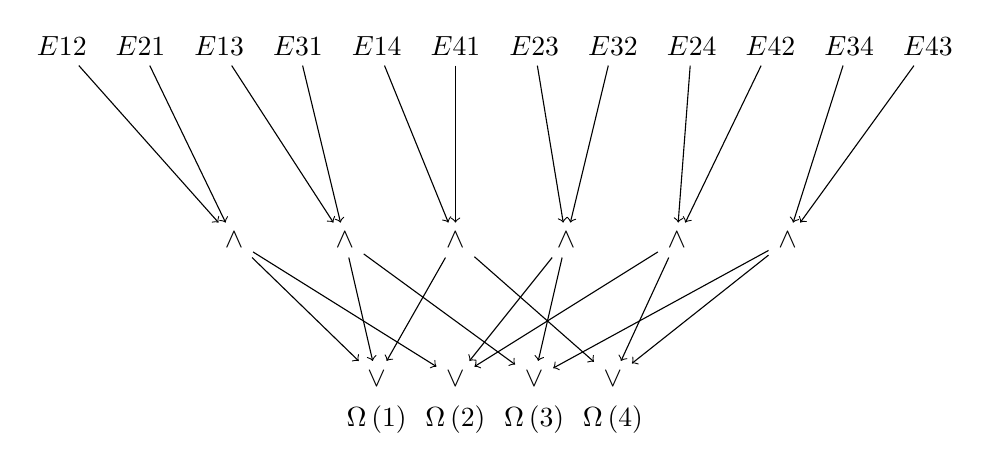
\begin{tikzpicture}

\node (E12) {$E 1 2$};
\node [right of=E12] (E21) {$E 2 1$};
\node [right of=E21] (E13) {$E 1 3$};
\node [right of=E13] (E31) {$E 3 1$};
\node [right of=E31] (E14) {$E 1 4$};
\node [right of=E14] (E41) {$E 4 1$};
\node [right of=E41] (E23) {$E 2 3$};
\node [right of=E23] (E32) {$E 3 2$};
\node [right of=E32] (E24) {$E 2 4$};
\node [right of=E24] (E42) {$E 4 2$};
\node [right of=E42] (E34) {$E 3 4$};
\node [right of=E34] (E43) {$E 4 3$};

\node [below of=E41,node distance=7em] (14) {$\wedge$};
\node [left of=14,node distance=4em] (13) {$\wedge$};
\node [left of=13,node distance=4em] (12) {$\wedge$};
\node [right of=14,node distance=4em] (23) {$\wedge$};
\node [right of=23,node distance=4em] (24) {$\wedge$};
\node [right of=24,node distance=4em] (34) {$\wedge$};

\node [below of=14,node distance=5em,label=below:$\Omega\left(2\right)$] (2) {$\vee$};
\node [left of=2,label=below:$\Omega\left(1\right)$] (1) {$\vee$};
\node [right of=2,label=below:$\Omega\left(3\right)$] (3) {$\vee$};
\node [right of=3,label=below:$\Omega\left(4\right)$] (4) {$\vee$};

\path [->]
		(E12) edge (12) (E21) edge (12)
		(E13) edge (13) (E31) edge (13)
		(E14) edge (14) (E41) edge (14)
		(E23) edge (23) (E32) edge (23)
		(E24) edge (24) (E42) edge (24)
		(E34) edge (34) (E43) edge (34)

		(12) edge (1) (12) edge (2)
		(13) edge (1) (13) edge (3)
		(14) edge (1) (14) edge (4)
		(23) edge (2) (23) edge (3)
		(24) edge (2) (24) edge (4)
		(34) edge (3) (34) edge (4)

;

\end{tikzpicture}
\par\end{centering}

\caption{Schaltkreis $\mathcal{C}_{4}$}


\end{figure}

\end{example*}

\subsection{Eigenschaften von Schaltkreisen}
\begin{defn}
\textbf{Invarianz}

Ein $k$-stelliger Schaltkreis $\mathcal{C}$ mit dem Universum $U$
heiße \textbf{invariant} wenn für alle $\mathfrak{A}\in\mathbf{FIN}_{<}\left(\sigma\right)$,
alle $\bar{a}\in A^{\mathrm{ar}\left(\mathcal{C}\right)}$ und alle
Bijektionen $\pi_{1},\pi_{2}:A\rightarrow U$ gilt:
\[
\mathcal{C}\left[\pi_{1}\mathfrak{A}\right]\left(\Omega\left(\pi_{1}\bar{a}\right)\right)=\mathcal{C}\left[\pi_{2}\mathfrak{A}\right]\left(\Omega\left(\pi{}_{2}\bar{a}\right)\right)
\]


Für invariante Schaltkreise und beliebige Strukturen $\mathfrak{A}\in\mathbf{FIN}\left(\sigma\right)$
bezeichne $\mathcal{C}\left[\mathfrak{A}\right]$ die Auswertung $\mathcal{C}\left[\pi\mathfrak{A}\right]$
mit einer beliebigen Bijektion $\pi:A\rightarrow U$.
\end{defn}

\begin{defn}
\textbf{Symmetrie}
\end{defn}
Ein Schaltkreis $\mathcal{C}=\left(G,W,\Sigma,\Omega,U\right)$ heiße
\textbf{symmetrisch}, wenn für jede Permutation der Universums $\pi\in\mathrm{Sym}_{U}$
ein Automorphismus $\hat{\pi}:G\rightarrow G$ des Graphen $\left(G,W\right)$
existiert, der die folgenden Bedingungen erfüllt:
\begin{enumerate}
\item Für alle Gates $g$ mit $\Sigma\left(g\right)=R\bar{x}$ gilt $\Sigma\left(\hat{\pi}g\right)=R\,\pi\bar{x}$.
\item Für alle übrigen Gates gilt $\Sigma\left(g\right)=\Sigma\left(\hat{\pi}g\right)$.
\item Für jedes Tupel $\bar{x}\in U$ gilt $\Omega\left(\pi\bar{x}\right)=\hat{\pi}\Omega\left(x\right)$.
\end{enumerate}
Falls jede Permutation von $U$ genau einen\emph{ }Automorphismus
induziert, so wird der von $\pi$ induzierte Automorphismus implizit
mit $\hat{\pi}$ notiert.
\begin{lem}
Symmetrie ist eine hinreichende, aber nicht notwendige, Bedingung
für die Invarianz eines Schaltkreises.\end{lem}
\begin{proof}
Sei $\mathcal{C}$ ein symmetrischer Schaltkreis, und $\mathfrak{A}$
eine beliebige Struktur mit $\left|A\right|=\left|U\right|$. Seien
$\pi_{1}$ und $\pi_{2}$ zwei beliebige Bijektionen von $A$ auf
$U$, und sei $\bar{a}\in A^{\mathrm{ar}\left(\mathcal{C}\right)}$
ein beliebiges Tupel. Es ist zu zeigen, dass: 
\[
\mathcal{C}\left[\pi_{1}\mathfrak{A}\right]\left(\Omega\left(\pi_{1}\bar{a}\right)\right)=\mathcal{C}\left[\pi_{2}\mathfrak{A}\right]\left(\Omega\left(\pi_{2}\bar{a}\right)\right)
\]


Wir definieren die Permutation $\tau:U\rightarrow U$ als $\tau\coloneqq\pi_{1}\pi_{2}^{-1}$,
so dass $\pi_{1}=\tau\pi_{2}$.

Per Voraussetzung induziert $\tau$ einen Automorphismus $\hat{\tau}$
auf $\mathcal{C}$: 
\begin{eqnarray*}
\hat{\tau}\left(W\right) & = & W\\
\Sigma\left(\hat{\tau}g\right) & = & \begin{cases}
R\tau\bar{x} & \mathrm{f\ddot{u}r}\,\Sigma\left(g\right)=R\bar{x}\\
\Sigma\left(g\right) & \mathrm{sonst}
\end{cases}\\
\Omega\left(\tau\bar{x}\right) & = & \hat{\tau}\Omega\left(\bar{x}\right)\,\mathrm{f\ddot{u}r\,alle}\,\bar{x}\in U^{\mathrm{ar}\left(\mathcal{C}\right)}
\end{eqnarray*}


Per Induktion über die Tiefe\footnote{Die Tiefe $T:G\rightarrow\mathbb{N}$ sei die maximale Länge eines
Weges von einer Quelle zum Gate $g$.} wird gezeigt: 
\begin{eqnarray*}
\mathcal{C}\left[\tau\pi_{2}\mathfrak{A}\right]\left(\hat{\tau}g\right)=\mathcal{C}\left[\pi_{2}\mathfrak{A}\right]\left(g\right) &  & \mathrm{f\ddot{u}r\,alle}\,g\in G
\end{eqnarray*}

\begin{description}
\item [{Induktionsanfang~$n=0$:}] Sei $g\in G$ eine Quelle mit $\Sigma\left(g\right)=R\bar{x}$.
Per Definition von $\tau$ und $\hat{\tau}$ gilt:
\[
\Sigma\left(\hat{\tau}g\right)=R\tau\bar{x}
\]
 
\begin{eqnarray*}
\tau\bar{x}\in\tau\pi_{2}R^{\mathfrak{A}} & \Longleftrightarrow & \bar{x}\in\pi_{2}R^{\mathfrak{A}}
\end{eqnarray*}
Es folgt: 
\[
\mathcal{C}\left[\tau\pi_{2}\mathfrak{A}\right]\left(\hat{\tau}g\right)=\mathcal{C}\left[\pi_{2}\mathfrak{A}\right]\left(g\right)
\]
(Falls $\Sigma\left(g\right)\in\left\{ \mathbf{0},\mathbf{1}\right\} $,
folgt die Behauptung direkt aus $\Sigma\left(\hat{\tau}g\right)=\Sigma\left(g\right)$.)
\item [{Induktionsschritt~$n\mapsto n+1$:}]~

\begin{description}
\item [{Annahme:}] Für alle Gates $g\in G$ mit Tiefe $T\left(g\right)\leqslant n$
gilt $\mathcal{C}\left[\tau\pi_{2}\mathfrak{A}\right]\left(\hat{\tau}g\right)=\mathcal{C}\left[\pi_{2}\mathfrak{A}\right]\left(g\right)$.
\end{description}

So gilt für jedes Gatter $g'\in G$ mit $T\left(g'\right)=n+1$: 
\begin{enumerate}
\item Die Beschriftungen $\Sigma\left(\hat{\tau}g'\right)=\Sigma\left(g'\right)=\phi$
sind gleich.
\item $\mathcal{C}\left[\tau\pi_{2}\mathfrak{A}\right]\left(\hat{\tau}g\right)=\mathcal{C}\left[\pi_{2}\mathfrak{A}\right]\left(g\right)$
für alle $\left(g,g'\right)\in W$.
\end{enumerate}

Es folgt $\mathcal{C}\left[\tau\pi_{2}\mathfrak{A}\right]\left(\hat{\tau}g'\right)=\mathcal{C}\left[\pi_{2}\mathfrak{A}\right]\left(g'\right)$.

\end{description}
Schließlich gilt für jedes Tupel $\bar{a}\in A^{\mathrm{ar}\left(\mathcal{C}\right)}$:

\begin{eqnarray*}
\mathcal{C}\left[\pi_{1}\mathfrak{A}\right]\left(\Omega\left(\pi_{1}\bar{a}\right)\right) & = & \mathcal{C}\left[\tau\pi_{2}\mathfrak{A}\right]\left(\Omega\left(\tau\pi_{2}\bar{a}\right)\right)\\
 & = & \mathcal{C}\left[\tau\pi_{2}\mathfrak{A}\right]\left(\hat{\tau}\Omega\left(\pi_{2}\bar{a}\right)\right)\\
 & = & \mathcal{C}\left[\pi_{2}\mathfrak{A}\right]\left(\Omega\left(\pi_{2}\bar{a}\right)\right)
\end{eqnarray*}


Damit ist der Schaltkreis invariant.
\end{proof}

\begin{proof}
Als Gegenbeispiel wird der folgende $0$-stellige Schaltkreis $\mathcal{C}$
über $U=\left\{ 1,2\right\} $ angeführt:

\begin{figure}[H]
\begin{centering}
\begin{center}
\tikzstyle{every node}=[circle, draw=black]
\begin{tikzpicture}

\node [label=below:$\Omega (\langle \rangle)$] (C) {$\wedge$};

\node [above left of=C,node distance=6em] (B1) {$\wedge$};


\node [above left of=B1,node distance=6em] (A1) {$E12$};
\node [right of=A1,node distance=5.5em] (A2) {$E11$};
\node [right of=B1,node distance=5.5em] (A3) {$E22$};
\node [right of=A3,node distance=5.5em] (A4) {$E21$};

\path [->] (A1) edge (B1) (A2) edge (B1) (A3) edge (C) (A4) edge (C)
			(B1) edge (C);
\end{tikzpicture}
\par\end{center}
\par\end{centering}

\caption{Schaltkreis}
\end{figure}

\end{proof}
Der Schaltkreis ist invariant, da er genau den Isomorphietyp $K_{2}$
akzeptiert. Er ist aber nicht symmetrisch: Die Permutation $\left(\begin{array}{cc}
1 & 2\\
2 & 1
\end{array}\right)$ induziert keinen Automorphismus.


\subsection{Eigenschaften von Schaltkreisfamilien}
\begin{defn}
Eine $\left(\sigma,\mathbb{B}\right)$-\textbf{Schaltkreisfamilie}
$\left(\mathcal{C}_{n}\right)_{n\in\mathbb{N}}$ sei eine Sequenz
von Schaltkreisen mit der gleichen Stelligkeit $\mathrm{ar}\left(\mathcal{C}_{n}\right)=k$
und den Universen $U^{\mathcal{C}_{n}}=\left\{ 1,\cdots,n\right\} $.

Eine invariante $\left(\sigma,\mathbb{B}\right)$-Schaltkreisfamilie
$\left(\mathcal{C}_{n}\right)_{n\in\mathbb{N}}$ \textbf{berechne}
eine $\sigma$-Anfrage $q$ genau dann wenn für alle $n\in\mathbb{N}$
und alle $\mathfrak{A}\in\mathbf{FIN}^{\left(n\right)}\left(\sigma\right)$
gilt: 
\[
q\left(\mathfrak{A}\right)=\mathcal{C}_{n}\left(\mathfrak{A}\right)
\]

\end{defn}

\begin{defn}
$\mathrm{SBC}$ und $\mathrm{SBC+\mathbf{MAJ}}$\end{defn}
\begin{itemize}
\item Sei $\mathrm{SBC}$ die Klasse aller \textbf{symmetrischen $\left(\sigma,\mathbb{B}_{\mathrm{std}}\right)$-Schaltkreisfamilien}.
\item Sei $\mathrm{SBC}+\mathbf{MAJ}$ die Klasse aller \textbf{symmetrischen
$\left(\sigma,\mathbb{B}_{\mathrm{maj}}\right)$-Schaltkreisfamilien}.
(Zur Erinnerung: $\mathbb{B}_{\mathrm{maj}}=\mathbb{B}_{\mathrm{std}}\uplus\left\{ \mathrm{MAJ}\right\} $,
wobei $\mathrm{MAJ}$ die Majority-Funktion ist.)
\end{itemize}

\begin{defn}
\textbf{Uniformität}

Für eine Zeitfunktion $T:\mathbb{N}\rightarrow\mathbb{N}$ sei eine
Schaltkreisfamilie $\mathcal{C}$ $T$-\textbf{uniform}, wenn eine
deterministische Turingmaschine bei Eingabe von $n\geqslant n_{0}$
eine Repräsentation von $\mathcal{C}_{n}$ in höchstens $T\left(n\right)$
Schritten berechnen kann.

Für eine Klasse von Zeitfunktionen $\mathscr{F}\subseteq\mathrm{Abb}\left(\mathbb{N},\mathbb{N}\right)$
sei sie $\mathscr{F}$-uniform, wenn ein $T\in\mathscr{F}$ existiert,
so dass sie $T$-uniform ist. Insbesondere sei $\mathrm{poly}\left(n\right)$
die Klasse aller polynomiell wachsenden Funktionen, und eine $\mathrm{poly}\left(n\right)$-uniforme
Schaltkreisfamilie heiße ,,P-uniform``.
\end{defn}

\begin{defn}
\textbf{Beschränkte Größe}

Für eine Funktion $f:\mathbb{N}\rightarrow\mathbb{N}$ habe eine Schaltkreisfamilie
$\mathcal{C}$ $f$-\textbf{Größe}, wenn jeder Schaltkreis $\mathcal{C}_{n}=\left(G,W,\Sigma,\Omega,U\right)$
höchstens $\left|G\right|\leqslant f\left(n\right)$ Gates besitzt.
Der Begriff ,,$\mathscr{F}$-groß`` sei analog zu ,,$\mathscr{F}$-uniform``
definiert.\end{defn}
\begin{rem*}
Es wird statt ,,$\mathrm{poly}\left(n\right)$-groß`` auch der Begriff
,,$\mathrm{P}/\mathrm{poly}$-uniform`` verwendet.

Eine $\mathrm{P/poly}$-Turingmaschine arbeitet mit einem polynomiell
beschränktem Orakel in Polynomialzeit, und kann daher genau solche
Schaltkreisfamilien berechnen, deren binäre Repräsentation polynomielle
Größe hat. Unter Voraussetzung einer geeigneten Kodierung sind dies
genau die $\mathrm{poly}\left(n\right)$-großen Schaltkreisfamilien.\end{rem*}
\begin{defn}
\textbf{Beschränkte Tiefe}

Für eine Funktion $f:\mathbb{N}\rightarrow\mathbb{N}$ sei eine Schaltkreisfamilie
$\mathcal{C}$ $f$-\textbf{Tiefe}, wenn jeder Schaltkreis $\mathcal{C}_{n}=\left(G,W,\Sigma,\Omega,U\right)$
höchstens $\left|G\right|\leqslant f\left(n\right)$ Gates besitzt.
Der Begriff ,,$\mathscr{F}$-tief`` sei analog zu ,,$\mathscr{F}$-groß``
definiert.\end{defn}
\begin{rem*}
$\mathrm{AC}^{0}$ ist die Klasse der $\mathcal{O}\left(1\right)$-tiefen,
$\mathrm{poly}\left(n\right)$-großen Schaltkreisfamilien.
\end{rem*}
\pagebreak{}


\section{Kernaussagen}


\subsection{Fixpunktlogiken und Schaltkreise}

Es werden die folgenden Äquivalenzen zwischen Fixpunktlogiken und
Schaltkreisklassen nachgewiesen:
\begin{thm}
\textbf{$\mathrm{FP}+\mathbf{ORD}$, $P$-uniforme $\mathrm{SBC}$}

Die folgenden Aussagen sind äquivalent:
\begin{enumerate}
\item Die Anfrage $q$ wird durch eine $\left(\mathrm{FP}+\mathbf{ORD}\right)\left[\sigma\right]$-Formel
$\varphi$ definiert.
\item Die Anfrage $q$ wird durch eine $P$-uniforme symmetrische $\left(\sigma,\mathbb{B}_{\mathrm{std}}\right)$-Schaltkreisfamilie
$\mathcal{C}$ berechnet.
\end{enumerate}
\end{thm}
Die Fixpunktlogik mit disjunkter Ordnungserweiterung und Zählterm
ist äquivalent zu den $P$-uniformen symmetrischen booleschen Schaltkreisfamilien
mit Majority-Gates.
\begin{thm}
\textbf{$\mathrm{FP}+C$, $P$-uniforme $\mathrm{SBC}+\mathbf{MAJ}$}

Die folgenden Aussagen sind äquivalent:
\begin{enumerate}
\item Die Anfrage $q$ wird durch eine $\left(\mathrm{FP}+C\right)\left[\sigma\right]$-Formel
$\varphi$ definiert.
\item Die Anfrage $q$ wird durch eine $P$-uniforme symmetrische $\left(\sigma,\mathbb{B}_{\mathrm{maj}}\right)$-Schaltkreisfamilie
$\mathcal{C}$ berechnet.
\end{enumerate}
\end{thm}
Zur Erinnerung: $\mathbb{B}_{\mathrm{maj}}$ enthält die boolesche
Konjunktion, Disjunktion und den Majority-Operator $\mathrm{MAJ}=\left\{ \left(m,n\right)\mid m\leqslant n\right\} $.


\begin{thm}
\textbf{$\mathrm{FP}+\Upsilon$, $\mathrm{poly\left(n\right)}$-große
$\mathrm{SBC}$}

Die folgenden Aussagen sind äquivalent:
\begin{enumerate}
\item Die Anfrage $q$ wird durch eine $\left(\mathrm{FP}+\Upsilon\right)\left[\sigma\right]$-Formel
$\varphi$ definiert.
\item Die Anfrage $q$ wird durch eine $\mathrm{poly}\left(n\right)$-große
symmetrische $\left(\sigma,\mathbb{B}_{\mathrm{std}}\right)$-Schaltkreisfamilie
$\mathcal{C}$ berechnet.
\end{enumerate}
\end{thm}
Zur Erinnerung: $\mathbb{B}_{\mathrm{maj}}$ enthält die boolesche
Konjunktion, Disjunktion und den Majority-Operator $\mathrm{MAJ}=\left\{ \left(m,n\right)\mid m\leqslant n\right\} $.


\begin{thm}
\textbf{$\mathrm{FP}+\Upsilon+C$, $\mathrm{poly}\left(n\right)$-große
$\mathrm{SBC}+\mathbf{MAJ}$}

Die folgenden Aussagen sind äquivalent:
\begin{enumerate}
\item Die Anfrage $q$ wird durch eine $\left(\mathrm{FP}+\Upsilon+C\right)\left[\sigma\right]$-Formel
$\varphi$ definiert.
\item Die Anfrage $q$ wird durch eine $\mathrm{poly}\left(n\right)$-große
symmetrische $\left(\sigma,\mathbb{B}_{\mathrm{maj}}\right)$-Schaltkreisfamilie
$\mathcal{C}$ berechnet.
\end{enumerate}
\end{thm}
eine Orakelfunktion, die jeder Zahl $n$ die Orakelstruktur $\mathbf{ARB}\left(n\right)=\mathfrak{N}_{\mid\left\{ 0,\cdots,n\right\} }$
zuweist.

Für jede $\mathrm{FO}+\mathbf{ARB}$-Formel $\varphi$ existiert eine
arb-invariante $\mathrm{FO}\left[\sigma_{\mathrm{arb}}\right]$-Formel
$\varphi'$, die auf allen endlichen $\sigma$-Strukturen äquivalent
zu $\varphi$ ist, und umgekehrt.


\subsection{FO-Logiken und Schaltkreise}
\begin{thm}
\label{thm:5.5:fo-ord}$\mathrm{FO}+\mathbf{ORD}$, $P$-uniformes
symmetrisches $\mathrm{AC}^{0}$.

Die folgenden Aussagen sind äquivalent:
\begin{enumerate}
\item Die Anfrage $q$ wird durch eine $\left(\mathrm{FO}+\mathbf{ORD}\right)\left[\sigma\right]$-Formel
$\varphi$ definiert.
\item Die Anfrage $q$ wird durch eine $P$-uniforme, $\mathcal{O}\left(1\right)$-tiefe,
symmetrische $\left(\sigma,\mathbb{B}_{\mathrm{std}}\right)$-Schaltkreisfamilie
$\mathcal{C}$ berechnet.
\end{enumerate}
\end{thm}

\begin{thm}
\label{thm:5.6:fo-c}$\mathrm{FO}+C$, symmetrisches $\mathrm{AC}^{0}+\mathbf{MAJ}$.

Die folgenden Aussagen sind äquivalent:
\begin{enumerate}
\item Die Anfrage $q$ wird durch eine $\left(\mathrm{FO}+C\right)\left[\sigma\right]$-Formel
$\varphi$ definiert.
\item Die Anfrage $q$ wird durch eine $\mathcal{O}\left(1\right)$-tiefe,
$\mathrm{poly}\left(n\right)$-große, symmetrische $\left(\sigma,\mathbb{B}_{\mathrm{maj}}\right)$-Schaltkreisfamilie
$\mathcal{C}$ berechnet.
\end{enumerate}
\end{thm}

\begin{thm}
\label{thm:5.7:fo+u}$\mathrm{FO}+\Upsilon$, symmetrisches $\mathrm{AC}^{0}$.

Die folgenden Aussagen sind äquivalent:
\begin{enumerate}
\item Die Anfrage $q$ wird durch eine $\left(\mathrm{FO}+\Upsilon\right)\left[\sigma\right]$-Formel
$\varphi$ definiert.
\item Die Anfrage $q$ wird durch eine $\mathcal{O}\left(1\right)$-tiefe,
$\mathrm{poly}\left(n\right)$-große, symmetrische $\left(\sigma,\mathbb{B}_{\mathrm{std}}\right)$-Schaltkreisfamilie
$\mathcal{C}$ berechnet.\end{enumerate}
\begin{thm}
$\mathrm{FO}+\Upsilon+C$, symmetrisches $\mathrm{AC}^{0}+\mathbf{MAJ}$.

Die folgenden Aussagen sind äquivalent:
\begin{enumerate}
\item Die Anfrage $q$ wird durch eine $\left(\mathrm{FO}+\Upsilon\right)\left[\sigma\right]$-Formel
$\varphi$ definiert.
\item Die Anfrage $q$ wird durch eine $\mathcal{O}\left(1\right)$-tiefe,
$\mathrm{poly}\left(n\right)$-große, symmetrische $\left(\sigma,\mathbb{B}_{\mathrm{maj}}\right)$-Schaltkreisfamilie
$\mathcal{C}$ berechnet.
\end{enumerate}
\end{thm}
\end{thm}

\subsection{FO-Logik mit disjunktem und nicht-disjunktem Orakel}
\begin{thm}
$\mathrm{FO}+\Upsilon$, invariantes $\mathrm{FO}\left(\mathrm{arb}\right)$
\begin{enumerate}
\item Jede $\left(\mathrm{FO}+\Upsilon\right)\left[\sigma\right]$-Formel
$\varphi$ ist äquivalent zu einer arb-invarianten $\mathrm{FO}\left[\sigma_{\mathrm{arb}}\right]$-Formel
$\varphi$.
\item Es existiert eine $\sigma$-Anfrage, die in der arb-invarianten $\mathrm{FO}\left[\sigma_{\mathrm{arb}}\right]$-Logik
definierbar ist, aber nicht $\left(\mathrm{FO}+\Upsilon\right)\left[\sigma\right]$-definierbar
ist.
\end{enumerate}
\end{thm}
\pagebreak{}


\section{Von Formeln zu Schaltkreisen}


\subsection{FO-Logik}

Die Formeln der Logik erster Stufe sind durch symmetrisches, $P$-uniformes
$\mathrm{AC}^{0}$ berechenbar:
\begin{defn*}
.\end{defn*}
\begin{lem}
\label{lem:FO-Circuit}Jede $\mathrm{FO}\left[\sigma\right]$-Formel
$\varphi$ definiert eine $\sigma$-Anfrage $q$, die von einer symmetrischen,
$P$-uniformen Schaltkreis-Familie $\left(\mathcal{C}_{n}^{\varphi}\right)_{n\in\mathbb{N}}$
mit konstanter Tiefe $T_{n}\leqslant3\left\Vert \varphi\right\Vert $
und polynomieller Größe $S_{n}\leqslant5\left\Vert \varphi\right\Vert n^{\mathtt{M}\left(\varphi\right)}$
berechnet wird.\end{lem}
\begin{proof}
Sei $\sigma$ eine relationale Signatur, und sei $\varphi\left(\bar{x}\right)$
eine $k$-stellige $\mathrm{FO}\left[\sigma\right]$-Formel.

Per induktiver Konstruktion über den Aufbau von $\varphi$ wird der
$k$-stellige Schaltkreis $\mathcal{C}_{n}^{\varphi}$ über dem Universum
$U\coloneqq\left\{ 1,\cdots,n\right\} $ definiert. Die Konstruktion
ist in Polynomialzeit berechenbar. Für eine beliebige Permutation
$\pi\in\mathrm{Sym}_{U}$ wird ein Automorphismus $\hat{\pi}$ angegeben.
\begin{casenv}
\item Falls $\varphi\left(\bar{x}\right)=R\bar{y}$ für $R\in\sigma$, so
besteht $\mathcal{C}_{n}^{\varphi}$ aus $n^{k}$ isolierten Gates.

\begin{description}
\item [{Schaltkreis:}] 
\[
\mathcal{C}_{n}^{\varphi}\coloneqq\left(\left\{ g_{\bar{t}}\mid\bar{t}\in U^{k}\right\} ,\emptyset,\Sigma,\Omega,U\right)
\]
Für jedes Tupel $\bar{t}\in U^{k}$ sei $\beta_{\bar{t}}\coloneqq\left(\begin{array}{c}
\bar{x}\\
\bar{t}
\end{array}\right)$ die Abbildung der Variablen $\bar{x}$ auf das Tupel $\bar{t}$:
\begin{eqnarray*}
\Omega\left(\bar{t}\right) & \coloneqq & g_{\bar{t}}\\
\Sigma\left(g_{\bar{t}}\right) & \coloneqq & R\beta_{\bar{t}}\left(\bar{y}\right)
\end{eqnarray*}

\item [{Korrektheit:}] Es gilt 
\[
\begin{array}{ccccc}
\left\llbracket R\bar{x}\right\rrbracket \left(\mathfrak{A},\bar{t}\right)=1 & \overset{\mathrm{def}}{\Leftrightarrow} & \bar{t}\in R^{\mathfrak{A}} & \overset{\mathrm{def}}{\Leftrightarrow} & \mathcal{C}_{n}^{\varphi}\left[\mathfrak{A}\right]\left(g_{\bar{t}}\right)=1\end{array}
\]

\item [{Symmetrie:}] Sei $\hat{\pi}g_{\bar{t}}\coloneqq g_{\pi\bar{t}}$
für alle Tupel $\bar{t}\in U^{m}$. Per Definition ist $\pi\beta_{\bar{t}}\left(\bar{y}\right)=\beta_{\pi\bar{t}}\left(\bar{y}\right)$
und daher sind die Markierungen $\Sigma\left(\hat{\pi}g_{\bar{t}}\right)=\pi\Sigma\left(g_{\bar{t}}\right)$
und $\Omega\left(\pi\bar{t}\right)=g_{\pi\bar{t}}=\hat{\pi}\Omega\left(\bar{t}\right)$.
\end{description}
\item Falls $\varphi\left(\bar{x}\right)=y_{1}\dot{=}y_{2}$, so besteht
$\mathcal{C}_{n}^{\varphi}$ aus $n^{k}$ isolierten Gates (hier ist
$k\in\left\{ 1,2\right\} $).

\begin{description}
\item [{Schaltkreis:}] 
\[
\mathcal{C}_{n}^{\varphi}\coloneqq\left(\left\{ g_{\bar{t}}\mid\bar{t}\in U^{k}\right\} ,\emptyset,\Sigma,\Omega,U\right)
\]
Für jedes Tupel $\bar{t}\in U^{k}$ sei $\beta_{\bar{t}}\coloneqq\left(\begin{array}{c}
\bar{x}\\
\bar{t}
\end{array}\right)$ die entsprechende Belegung:
\begin{eqnarray*}
\Omega\left(\bar{t}\right) & \coloneqq & g_{\bar{t}}\\
\Sigma\left(g_{\bar{t}}\right) & \coloneqq & \begin{cases}
\mathbf{1} & \mathrm{falls}\,\beta\left(y_{1}\right)=\beta\left(y_{2}\right)\\
\mathbf{0} & \mathrm{sonst}
\end{cases}
\end{eqnarray*}

\item [{Korrektheit:}] Es gilt 
\[
\begin{array}{ccccc}
\left\llbracket y_{1}\dot{=}y_{2}\right\rrbracket \left(\mathfrak{A},\bar{t}\right)=1 & \overset{\mathrm{def}}{\Leftrightarrow} & \beta_{\bar{t}}y_{1}=\beta_{\bar{t}}y_{2} & \overset{\mathrm{def}}{\Leftrightarrow} & \mathcal{C}_{n}^{\varphi}\left[\mathfrak{A}\right]\left(g_{\bar{t}}\right)=1\end{array}
\]

\item [{Symmetrie:}] Sei $\hat{\pi}\left(g_{\bar{t}}\right)\coloneqq g_{\pi\bar{t}}$.
Es gilt $\beta_{\bar{t}}\left(x\right)=\beta_{\bar{t}}\left(x'\right)$
genau dann wenn $\beta_{\pi\bar{t}}\left(x\right)=\beta_{\pi\bar{t}}\left(x\right)$,
und daher ist $\Sigma\left(\hat{\pi}g_{\bar{t}}\right)=\Sigma\left(g_{\pi\bar{t}}\right)$.
\end{description}
\item Falls $\varphi\left(\bar{x}\right)=\varphi_{1}\left(\bar{y_{1}}\right)\wedge\cdots\wedge\varphi_{m}\left(\bar{y_{m}}\right)$
mit $\mathrm{ar}\left(\varphi_{i}\right)=k_{i}$, so besteht $\mathcal{C}_{n}^{\varphi}$
aus der disjunkten Vereinigung aller $\mathcal{C}_{n}^{\varphi_{i}}$
für $1\leqslant i\leqslant m$ mit der folgenden Erweiterung.

\begin{description}
\item [{Schaltkreis:}] 
\begin{eqnarray*}
\mathcal{C}_{n}^{\varphi} & \coloneqq & \left(G,W,\Sigma,\Omega,U\right)\\
\mathcal{C}_{n}^{\varphi_{i}} & = & \left(G_{i},W_{i},\Sigma_{i},\Omega_{i},U\right)
\end{eqnarray*}
 werden neue Outputs für jedes $k$-Tupel aus $U$ hinzugefügt:
\begin{eqnarray*}
G & \coloneqq & \biguplus_{i=1}^{\ell}G_{i}\uplus\left\{ g_{\bar{t}}\mid\bar{t}\in U^{k}\right\} 
\end{eqnarray*}
Die Outputs werden entsprechend mit denen der Teilschaltkreise verknüpft,
wobei $\rho_{i}:U^{k}\rightarrow U^{k_{i}}$ ein $k$-Tupel $\bar{t}$
wie folgt auf die in $\varphi_{i}$ frei vorkommenden Variablen reduziere:
\[
\mathrm{Sei}\,\left(\left(y_{i}\right)_{1},\cdots,\left(y_{i}\right)_{k_{i}}\right)=\left(x_{\left(j_{1}\right)},\cdots,x_{\left(j_{k_{i}}\right)}\right)
\]
\begin{eqnarray*}
\rho_{i}\left(t_{1},\cdots,t_{k}\right) & \coloneqq & \left(t_{\left(j_{1}\right)},\cdots,t_{\left(j_{k_{i}}\right)}\right)
\end{eqnarray*}
\[
W\coloneqq\biguplus_{i=1}^{\ell}W_{i}\uplus\left\{ \left(\Omega_{i}\left(\rho_{i}\bar{t}\right),g_{\bar{t}}\right)\mid1\leqslant i\leqslant\ell,\,\bar{t}\in U^{m}\right\} 
\]
Die Gates werden entsprechend beschriftet:
\begin{eqnarray*}
\Sigma\left(g\right) & \coloneqq & \begin{cases}
\Sigma_{i}\left(g\right) & \mathrm{f\ddot{u}r}\,g\in G_{i}\\
\wedge & \mathrm{sonst}
\end{cases}\\
\Omega\left(\bar{t}\right) & \coloneqq & g_{\bar{t}}\,\,\mathrm{f\ddot{u}r\,alle\,\,}\bar{t}\in U^{m'}
\end{eqnarray*}

\item [{Korrektheit:}] Es gilt 
\begin{eqnarray*}
\left\llbracket \varphi_{1}\wedge\cdots\wedge\varphi_{k}\right\rrbracket \left(\mathfrak{A},\bar{t}\right) & = & \min_{1\leqslant i\leqslant k}\left\llbracket \varphi_{i}\right\rrbracket \left(\mathfrak{A},\bar{t}\right)\\
 & = & \min_{1\leqslant i\leqslant k}\mathcal{C}_{n}^{\varphi_{i}}\left[\mathfrak{A}\right]\left(\Omega_{i}\left(\rho_{i}\bar{t}\right)\right)\\
 & = & \mathcal{C}_{n}^{\varphi}\left[\mathfrak{A}\right]\left(g_{\bar{t}}\right)
\end{eqnarray*}

\item [{Symmetrie:}] Es existieren bereits die Automorphismen $\hat{\pi_{i}}$
für jeden Schaltkreis $\mathcal{C}_{n}^{\varphi_{i}}$. Der Automorphismus
$\hat{\pi}$ erweitert diese:
\[
\hat{\pi}\left(g\right)\coloneqq\begin{cases}
\hat{\pi}_{i}\left(g\right) & \mathrm{f\ddot{u}r}\,g\in G_{i}\\
g_{\pi\bar{t}} & \mathrm{f\ddot{u}r}\,g=g_{\bar{t}}
\end{cases}
\]
Für die Gates und Kanten der Schaltkreise $\mathcal{C}_{n}^{\varphi_{i}}$
ist $\hat{\pi}$ per Annahme bereits korrekt.\end{description}
\begin{enumerate}
\item Für die neuen Kanten $\left(\Omega_{i}\left(\rho_{i}\bar{t}\right),g_{\bar{t}}\right)\in W$
gilt nach Voraussetzung: 
\begin{eqnarray*}
\left(\hat{\pi}\Omega_{i}\left(\rho_{i}\bar{t}\right),\hat{\pi}g_{\bar{t}}\right) & = & \left(\hat{\pi}_{i}\Omega_{i}\left(\rho_{i}\bar{t}\right),\hat{\pi}g_{\bar{t}}\right)\\
 & = & \left(\Omega_{i}\left(\pi\rho_{i}\bar{t}\right),g_{\pi\bar{t}}\right)\\
 & = & \left(\Omega_{i}\left(\rho_{i}\pi\bar{t}\right),g_{\pi\bar{t}}\right)\in W
\end{eqnarray*}
(Die Abbildung $\rho_{i}:U^{m}\rightarrow U^{m_{i}}$ ist ein Homomorphismus
und kommutiert mit der Permutation $\pi$.)
\item Es gilt $\Sigma\left(\hat{\pi}g_{\bar{t}}\right)=\Sigma\left(g_{\bar{t}}\right)=\vee$.
\item Es gilt $\Omega\left(\pi\bar{t}\right)=g_{\pi\bar{t}}=\hat{\pi}gv=\hat{\pi}\Omega\left(\bar{t}\right)$.
\end{enumerate}
\item Falls $\varphi\left(\bar{x}\right)=\varphi_{1}\vee\cdots\vee\varphi_{\ell}$,
so ist der Schaltkreis analog zu Fall 3 mit $\Sigma\left(g_{\bar{t}}\right)=\vee$.
\item Falls $\varphi\left(\bar{x}\right)=\neg\psi$, so wird der Schaltkreis
$\mathcal{C}_{n}^{\psi}$ wie folgt erweitert:

\begin{description}
\item [{Schaltkreis:}] 
\begin{eqnarray*}
\mathcal{C}_{n}^{\psi} & = & \left(G',W',\Sigma',\Omega',U\right)\\
\mathcal{C}_{n}^{\varphi} & \coloneqq & \left(G,W,\Sigma,\Omega,U\right)
\end{eqnarray*}
Für jedes Tupel $\bar{t}\in U^{m}$ wird ein neues Gate $g_{\bar{t}}$
eingefügt. Die Gates werden mit den Outputs von $\mathcal{C}_{n}^{\varphi'}$
verknüpft. 
\begin{eqnarray*}
G & \coloneqq & G'\uplus\left\{ g_{\bar{t}}\mid\bar{t}\in U^{m}\right\} \\
W & \coloneqq & W'\uplus\left\{ \left(\Omega'\left(\bar{t}\right),g_{\bar{t}}\right)\mid\bar{t}\in U^{m}\right\} \\
\Sigma\left(g\right) & \coloneqq & \begin{cases}
\Sigma'\left(g\right) & \mathrm{falls}\,g\in G'\\
\neg & \mathrm{sonst}
\end{cases}\\
\Omega\left(\bar{t}\right) & \coloneqq & g_{\bar{t}}
\end{eqnarray*}

\item [{Korrektheit:}] Es gilt 
\begin{eqnarray*}
\left\llbracket \neg\psi\right\rrbracket \left(\mathfrak{A},\bar{t}\right) & = & 1-\left\llbracket \psi\right\rrbracket \left(\mathfrak{A},\bar{t}\right)\\
 & = & 1-\mathcal{C}_{n}^{\psi}\left[\mathfrak{A}\right]\left(\Omega'\left(\bar{t}\right)\right)\\
 & = & \mathcal{C}_{n}^{\varphi}\left[\mathfrak{A}\right]\left(g_{\bar{t}}\right)
\end{eqnarray*}

\item [{Symmetrie:}] Es existiert bereits der Automorphismus $\hat{\pi'}$.
Dieser wird wie folgt erweitert:
\[
\hat{\pi}\left(g\right)\coloneqq\begin{cases}
\hat{\pi'}\left(g\right) & \mathrm{falls}\,g\in G'\\
g_{\pi\bar{t}} & \mathrm{falls}\,g=g_{\bar{t}}
\end{cases}
\]

\end{description}
\item Falls $\varphi\left(\bar{x}\right)=\left(\varphi_{1}\rightarrow\varphi_{2}\right)$,
so ist der Schaltkreis $\mathcal{C}_{n}^{\varphi}\coloneqq\mathcal{C}_{n}^{\left(\neg\varphi_{1}\vee\varphi_{2}\right)}$.
\item Falls $\varphi\left(\bar{x}\right)=\left(\varphi_{1}\left(\bar{y_{1}}\right)\leftrightarrow\varphi_{2}\left(\bar{y_{2}}\right)\right)$,
so besteht $\mathcal{C}_{n}^{\varphi}$ aus der disjunkten Vereinigung
von $\mathcal{C}_{n}^{\varphi_{1}}$ und $\mathcal{C}_{n}^{\varphi_{2}}$
mit der folgenden Erweiterung:
\begin{eqnarray*}
\mathcal{C}_{n}^{\varphi} & \coloneqq & \left(G,W,\Sigma,\Omega,U\right)\\
\mathcal{C}_{n}^{\varphi_{i}} & \coloneqq & \left(G_{i},W_{i},\Sigma_{i},\Omega_{i},U\right)
\end{eqnarray*}


\begin{description}
\item [{Schaltkreis:}] Für jedes Tupel $\bar{t}\in U^{m}$ werden fünf
neue Gates eingefügt:
\begin{eqnarray*}
G & \coloneqq & G_{1}\uplus G_{2}\\
 &  & \uplus\left\{ a_{\bar{t}},b_{\bar{t}},c_{\bar{t}},d_{\bar{t}},e_{\bar{t}}\mid\bar{t}\in U^{m}\right\} 
\end{eqnarray*}
Die Gates $a_{\bar{t}}$ und $b_{\bar{t}}$ negieren die Schaltkreise
$\mathcal{C}_{n}^{\varphi_{1}}$ und $\mathcal{C}_{n}^{\varphi_{2}}$.
Die Gates $\bar{c}_{t}$ und $\bar{d_{t}}$ sind Konjunktionen von
$\left(\varphi_{1}\wedge\varphi_{2}\right)$ und $\left(\neg\varphi_{1}\wedge\neg\varphi_{2}\right)$.
Die Gates $e_{\bar{t}}$ sind die Disjunktionen von $c_{\bar{t}}$
und $d_{\bar{t}}$. 
\begin{eqnarray*}
W & \coloneqq & W_{1}\uplus W_{2}\\
 & \uplus & \left\{ \begin{array}{c}
\left(\Omega_{1}\left(\rho_{1}\bar{t}\right),a_{\rho_{1}\bar{t}}\right),\,\left(\Omega_{2}\left(\rho_{2}\bar{t}\right),b_{\rho_{2}\bar{t}}\right),\\
\left(\Omega_{1}\left(\rho_{1}\bar{t}\right),c_{\bar{t}}\right),\,\left(\Omega_{2}\left(\rho_{2}\bar{t}\right),c_{\bar{t}}\right),\\
\left(a_{\rho_{1}\bar{t}},d_{\bar{t}}\right),\,\left(b_{\rho_{2}\bar{t}},d_{\bar{t}}\right),\\
\left(c_{\bar{t}},e_{\bar{t}}\right),\,\left(d_{\bar{t}},e_{\bar{t}}\right)
\end{array}\mid\bar{t}\in U^{m}\right\} 
\end{eqnarray*}
(Hierbei seien $\rho_{1}$ und $\rho_{2}$ analog zu Fall 3 definiert.)
\begin{eqnarray*}
\Sigma\left(g\right) & \coloneqq & \begin{cases}
\neg & \mathrm{f\ddot{u}r}\,g\in\left\{ a_{\rho_{1}\bar{t}},b_{\rho_{2}\bar{t}}\mid\bar{t}\in U^{m}\right\} \\
\wedge & \mathrm{f\ddot{u}r}\,g\in\left\{ c_{\bar{t}},d_{\bar{t}}\mid\bar{t}\in U^{m}\right\} \\
\vee & \mathrm{f\ddot{u}r}\,g\in\left\{ e_{\bar{t}}\mid\bar{t}\in U^{m}\right\} \\
\Sigma_{i}\left(g\right) & \mathrm{f\ddot{u}r}\,g\in G_{i}
\end{cases}
\end{eqnarray*}
\[
\Omega\left(\bar{t}\right)=e_{\bar{t}}
\]

\item [{Korrektheit:}] Es gilt 
\begin{eqnarray*}
\left\llbracket \varphi\right\rrbracket \left(\mathfrak{A},\bar{t}\right) & = & \left\llbracket \left(\varphi_{1}\wedge\varphi_{2}\right)\vee\left(\neg\varphi_{1}\wedge\neg\varphi_{2}\right)\right\rrbracket \left(\mathfrak{A},\bar{t}\right)\\
 & = & \max\left(\begin{array}{c}
\min\left(\left\llbracket \varphi_{1}\right\rrbracket \left(\mathfrak{A},\bar{t}\right),\left\llbracket \varphi_{2}\right\rrbracket \left(\mathfrak{A},\bar{t}\right)\right),\\
\min\left(1-\left\llbracket \varphi_{1}\right\rrbracket \left(\mathfrak{A},\bar{t}\right),1-\left\llbracket \varphi_{2}\right\rrbracket \left(\mathfrak{A},\bar{t}\right)\right)
\end{array}\right)\\
 & = & \max\left(\begin{array}{c}
\min\left(\mathcal{C}_{n}^{\varphi}\left[\mathfrak{A}\right]\left(\Omega_{1}\left(\rho_{1}\bar{t}\right)\right),\mathcal{C}_{n}^{\varphi}\left[\mathfrak{A}\right]\left(\Omega_{2}\left(\rho_{2}\bar{t}\right)\right)\right),\\
\min\left(1-\mathcal{C}_{n}^{\varphi}\left[\mathfrak{A}\right]\left(\Omega_{1}\left(\rho_{1}\bar{t}\right)\right),1-\mathcal{C}_{n}^{\varphi}\left[\mathfrak{A}\right]\left(\Omega_{2}\left(\rho_{2}\bar{t}\right)\right)\right)
\end{array}\right)\\
 & = & \max\left(\begin{array}{c}
\mathcal{C}_{n}^{\varphi}\left[\mathfrak{A}\right]\left(c_{t}\right),\\
\min\left(\mathcal{C}_{n}^{\varphi}\left[\mathfrak{A}\right]\left(a_{\rho_{1}\bar{t}}\right),\mathcal{C}_{n}^{\varphi}\left[\mathfrak{A}\right]\left(b_{\rho_{2}\bar{t}}\right)\right)
\end{array}\right)\\
 & = & \max\left(\mathcal{C}_{n}^{\varphi}\left[\mathfrak{A}\right]\left(c_{t}\right),\mathcal{C}_{n}^{\varphi}\left[\mathfrak{A}\right]\left(d_{\bar{t}}\right)\right)\\
 & = & \mathcal{C}_{n}^{\varphi}\left[\mathfrak{A}\right]\left(e_{\bar{t}}\right)
\end{eqnarray*}

\item [{Symmetrie:}] Es existieren per Annahme die Automorphismen $\hat{\pi_{i}}$
für die Schaltkreise $\mathcal{C}_{n}^{\varphi_{i}}$. Diese werden
wie folgt erweitert:
\[
\hat{\pi}\left(g\right)\coloneqq\begin{cases}
\hat{\pi_{i}}\left(g\right) & \mathrm{f\ddot{u}r}\,g\in G_{i}\\
g_{\pi\bar{t}} & \mathrm{f\ddot{u}r}\,g=g_{\bar{t}}\,\mathrm{und}\,g\in\left\{ a,b,c,d,e\right\} 
\end{cases}
\]

\end{description}
\item Falls $\varphi\left(\bar{x}\right)=\exists y_{1}\cdots\exists y_{m}\psi\left(z_{1},\cdots,z_{k+m}\right)$,
so wird der Schaltkreis $\mathcal{C}_{n}^{\varphi'}$ wie folgt erweitert:

\begin{description}
\item [{Schaltkreis:}] 
\begin{eqnarray*}
\mathcal{C}_{n}^{\varphi} & \coloneqq & \left(G,W,\Sigma,\Omega,U\right)\\
\mathcal{C}_{n}^{\varphi'} & \coloneqq & \left(G',W',\Sigma',\Omega',U\right)
\end{eqnarray*}
Sei $\rho:U^{k+m}\rightarrow U^{k}$ die Abbildung, die $\bar{z}$
auf die freien Variablen $\bar{x}$ reduziere:
\begin{eqnarray*}
\left(x_{1},\cdots,x_{k}\right) & = & \left(z_{\left(i_{i}\right)},\cdots,z_{\left(i_{k}\right)}\right)\\
\rho\left(t_{1},\cdots,t_{k+m}\right) & \coloneqq & \left(t_{\left(i_{1}\right)},\cdots,t_{\left(i_{k}\right)}\right)
\end{eqnarray*}

\end{description}

Es werden neue Outputs eingefügt:
\begin{eqnarray*}
G & \coloneqq & G'\uplus\left\{ g_{\bar{t}}\mid\bar{t}\in U^{k}\right\} 
\end{eqnarray*}
\[
\Omega\left(\bar{t}\right)\coloneqq g_{\bar{t}}
\]



Die neuen Outputs werden mit $\vee$ markiert.
\begin{eqnarray*}
\Sigma\left(g\right) & \coloneqq & \begin{cases}
\Sigma'\left(g\right) & \mathrm{f\ddot{u}r}\,g\in G'\\
\vee & \mathrm{sonst}
\end{cases}
\end{eqnarray*}
Jedes Gate $\Omega'\left(\bar{u}\right)$ mit $\bar{u}\in U^{k+m}$
wird mit dem Gate $g_{\rho\bar{u}}$ verknüpft:
\[
W\coloneqq W'\uplus\left\{ \left(\Omega'\left(\bar{u}\right),g_{\rho\bar{u}}\right)\mid\bar{u}\in U^{k+m}\right\} 
\]

\begin{description}
\item [{Korrektheit:}] Es gilt für 
\begin{eqnarray*}
\left\llbracket \varphi\right\rrbracket \left(\mathfrak{A},\bar{t}\right) & = & \max_{\begin{subarray}{c}
\bar{u}\in U^{k+m}\\
\rho\bar{u}=\bar{t}
\end{subarray}}\left\llbracket \psi\right\rrbracket \left(\mathfrak{A},\bar{u}\right)\\
 & = & \max_{\begin{subarray}{c}
\bar{u}\in U^{k+m}\\
\rho\bar{u}=\bar{t}
\end{subarray}}\left(\mathcal{C}_{n}^{\varphi}\left[\mathfrak{A}\right]\left(\Omega'\left(\bar{u}\right)\right)\right)\\
 & = & \mathcal{C}_{n}^{\varphi}\left[\mathfrak{A}\right]\left(g_{\bar{t}}\right)
\end{eqnarray*}

\item [{Symmetrie:}] Es existiert bereits der Automorphismus $\hat{\pi'}$.
Dieser wird wie folgt erweitert:
\[
\hat{\pi}\left(g\right)\coloneqq\begin{cases}
\hat{\pi'}\left(g\right) & \mathrm{f\ddot{u}r}\,g\in G'\\
g_{\pi\bar{t}} & \mathrm{f\ddot{u}r}\,g=g_{\bar{t}}
\end{cases}
\]
Auf den Gates von $\mathcal{C}_{n}^{\varphi'}$ ist $\hat{\pi}$ per
Annahme treu zu $\pi$.

\begin{enumerate}
\item Für die neuen Kanten $\left(\Omega'\left(\bar{u}\right),g_{\rho\bar{u}}\right)\in W$
gilt: $\left(\hat{\pi}\Omega'\left(\bar{u}\right),\hat{\pi}g_{\rho\bar{u}}\right)=\left(\Omega'\left(\pi\bar{u}\right),g_{\rho\pi\bar{u}}\right)\in W$.
\item $\hat{\pi}\Sigma\left(g_{\bar{t}}\right)=\Sigma\left(g_{\bar{t}}\right)=\vee$.
\item $\Omega\left(\pi\bar{t}\right)=g_{\pi\bar{t}}=\hat{\pi}g_{\bar{t}}=\hat{\pi}\Omega\left(\bar{t}\right)$.
\end{enumerate}
\end{description}
\item Falls $\varphi\left(\bar{x}\right)=\forall y_{1}\cdots\forall y_{m}\psi\left(\bar{z}\right)$,
so sei der Schaltkreis analog zu Fall 8 mit $\Sigma\left(g_{\bar{t}}\right)\coloneqq\wedge$.
\end{casenv}
Der so konstruierte Schaltkreis hat eine durch $3\left\Vert \varphi\right\Vert $
beschränkte Tiefe und eine durch $5\left\Vert \varphi\right\Vert \cdot n^{\mathtt{M}\left(\varphi\right)}$
beschränkte Größe. Dies folgt direkt aus der Tatsache, dass höchstens
$\left\Vert \varphi\right\Vert $ Induktionsschritte durchgeführt
werden, und jeder Schritt für eine $k$-stellige Teilformel die Tiefe
um maximal $3$ Kanten verlängert, und maximal $5n^{k}$ Gates hinzufügt.
(Insbesondere erreicht nur Fall 7 diese Schranken.)
\end{proof}
\pagebreak{}


\subsection{Ordnungserweiterung}

Wir betrachten die Logik $\mathrm{FO}+\mathbf{ORD}$, und weisen nach,
dass die Konstruktion aus Lemma \ref{lem:FO-Circuit} angepasst werden
kann.
\begin{lem}
\label{lem:fo-ord}Jede $\left(\mathrm{FO}+\mathbf{ORD}\right)\left[\sigma\right]$-Formel
$\varphi$ definiert eine $\sigma$-Anfrage $q$, die von einer symmetrischen,
$P$-uniformen $\left(\sigma,\mathbb{B}_{\mathrm{std}}\right)$-Schaltkreisfamilie
$\left(\mathcal{C}_{n}\right){}_{n\in\mathbb{N}}$ mit konstanter
Tiefe $T_{n}\leqslant3\left\Vert \varphi\right\Vert $ und polynomieller
Größe $S_{n}\leqslant5\left\Vert \varphi\right\Vert \left(2n+1\right)^{\mathtt{M}\left(\varphi\right)}$
berechnet wird.
\end{lem}
(Dieses Lemma bildet die erste Hälfte des Theorems \ref{thm:5.5:fo-ord}.)
\begin{proof}
Der Schaltkreis $\mathcal{C}_{n}$ wird über einer geordneten Struktur
$\mathfrak{A}\in\mathbf{FIN}_{<}\left(\sigma\right)$ über dem Universum
$U=\left\{ 1,\cdots,n\right\} $ ausgewertet.

Hierbei ist zu beachten, dass $U=\left\{ 1,\cdots,n\right\} $ keinesfalls
mit dem Universum der Orakelstruktur $\Upsilon\left(n\right)$ gleichzusetzen
ist!

Zur Unterscheidung verwenden wir die Umbenennung $\varodot:=\left(\begin{array}{c}
0,\cdots,n\\
\dot{0},\cdots,\dot{n}
\end{array}\right)$ und betrachten nur $\varodot\Upsilon\left(n\right)=\left(N,\leqslant\right)$.

Wir konstruieren zunächst den $\left(\sigma\uplus\left\{ \dot{\leqslant}\right\} ,\mathbb{B}_{\mathrm{std}}\right)$-Schaltkreis
$\mathcal{C}_{2n+1}^{\varphi}$ über $U=\left\{ 1,\cdots,2n+1\right\} $
entsprechend dem vorhergehenden Beweis. Dieser hat offensichtlich
die geforderte Größe $S_{n}=S_{2n+1}'=5\left\Vert \varphi\right\Vert \left(2n+1\right)^{\mathtt{M}\left(\varphi\right)}$.

Daraus wird der $\left(\sigma\uplus\left\{ \dot{\leqslant}\right\} ,\mathbb{B}_{\mathrm{std}}\right)$-Schaltkreis
$\dot{\mathcal{C}_{2n+1}^{\varphi}}=\left(G,W,\dot{\Sigma},\dot{\Omega},\dot{U}\right)$
über $\dot{U}=\left\{ 1,\cdots,n\right\} \uplus N$, in dem das Universum
durch $\rho:U\rightarrow\dot{U}$ umbenannt wird: 
\begin{eqnarray*}
\rho & \coloneqq & \left(\begin{array}{c}
1\\
1
\end{array}\cdots\begin{array}{c}
n\\
n
\end{array}\begin{array}{c}
\begin{array}{c}
n+1\\
\dot{0}
\end{array}\cdots\begin{array}{c}
2n+1\\
\dot{n}
\end{array}\end{array}\right)
\end{eqnarray*}
\[
\dot{\mathcal{C}_{2n+1}^{\varphi}}\coloneqq\rho\mathcal{C}_{2n+1}^{\varphi}=\left(G,W,\rho\Sigma,\Omega\rho,\rho U\right)
\]


Anschließend konstruieren wir daraus den $\left(\sigma,\mathbb{B}_{\mathrm{std}}\right)$-Schaltkreis
$\ddot{\mathcal{C}_{n}^{\varphi}}=\left(G,W,\ddot{\Sigma},\ddot{\Omega},\ddot{U}\right)$
über $\ddot{U}=\left\{ 1,\cdots,n\right\} $, indem alle Beschriftungen
$\dot{\Sigma}\left(g\right)=R\bar{t}$ mit $\bar{t}\notin\ddot{U}^{k}$
oder $R\notin\sigma$ durch $\ddot{\Sigma}\left(g\right)\in\left\{ \mathbf{0},\mathbf{1}\right\} $
ersetzt werden, und die Ausgangsfunktion auf $\ddot{\Omega}=\dot{\Omega}_{\mid\ddot{U}}$
reduziert wird.
\begin{casenv}
\item Für $\dot{\Sigma}\left(g\right)=R\bar{t}$ mit $R\in\sigma$ gilt:
\begin{eqnarray*}
\ddot{\Sigma}\left(g\right) & \coloneqq & \begin{cases}
R\bar{t} & \mathrm{falls}\,\bar{t}\in\ddot{U}^{k}\\
\mathbf{0} & \mathrm{sonst}
\end{cases}
\end{eqnarray*}

\item Für $\dot{\Sigma}\left(g\right)=t_{1}\dot{\leqslant}t_{2}$ gilt:
\begin{eqnarray*}
\ddot{\Sigma}\left(g\right) & \coloneqq & \begin{cases}
\mathbf{1} & \mathrm{falls}\,t_{1},t_{2}\in N,\,t_{1}\leqslant t_{2}\\
\mathbf{0} & \mathrm{sonst}
\end{cases}
\end{eqnarray*}

\end{casenv}
Sei nun $\ddot{\pi}\in\mathrm{Sym}_{\ddot{U}}$ eine beliebige Permutation.

Wir betrachten die Erweiterung $\dot{\pi}\coloneqq\ddot{\pi}\uplus\mathbf{id}_{\mid N}$,
die die Elemente von $N$ auf sich selbst abbildet. Offensichtlich
ist $\dot{\pi}\in\mathrm{Sym}_{\dot{U}}$ eine Permutation von $\dot{U}=\left(\ddot{U}\uplus N\right)$.

Entsprechend ist $\pi\coloneqq\rho^{-1}\dot{\pi}\in\mathrm{Sym}_{U}$
eine Permutation von $U=\left\{ 1,\cdots,2n+1\right\} $ mit $\pi_{\mid\left\{ n+1,\cdots,2n+1\right\} }=\mathbf{id}$.

Aus der Symmetrie des Schaltkreises $\mathcal{C}_{2n+1}^{\varphi}$
bezüglich $\mathrm{Sym}_{U}$ (siehe Lemma \ref{lem:FO-Circuit})
folgt die Existenz eines induzierten Automorphismus $\hat{\pi}$ für
den Schaltkreis $\mathcal{C}_{2n+1}^{\varphi}$. Wegen der Bijektivität
von $\rho$ wird $\hat{\pi}$ auch in $\rho\mathcal{C}_{2n+1}^{\varphi}=\dot{\mathcal{C}_{2n+1}^{\varphi}}$
durch $\dot{\pi}$ induziert.

Schließlich ist $\hat{\pi}$ auch in $\ddot{\mathcal{C}_{n}^{\varphi}}$
ein durch $\ddot{\pi}$ induzierter Automorphismus, wozu nur die Funktion
$\ddot{\Sigma}$ betrachtet werden muss (denn für $\ddot{\Omega}$
folgt die Symmetrie aus der Abgeschlossenheit von $\ddot{U}$ unter
$\ddot{\pi}$):
\begin{casenv}
\item Für $\varphi\left(\bar{x}\right)=R\bar{y}$ mit $R\in\sigma$ gilt:
\[
\ddot{\Sigma}\left(\hat{\pi}g_{\bar{t}}\right)=\ddot{\Sigma}\left(g_{\ddot{\pi}\bar{t}}\right)=\begin{cases}
\mathbf{1} & \mathrm{falls}\,\ddot{\pi}\bar{t},\bar{t}\in\ddot{U}^{k}\\
\mathbf{0} & \mathrm{sonst}
\end{cases}=\ddot{\Sigma}\left(g_{\bar{t}}\right)
\]

\item Für $\varphi\left(\bar{x}\right)=y_{1}\dot{=}y_{2}$ gilt:
\begin{eqnarray*}
\ddot{\Sigma}\left(\hat{\pi}g_{\bar{t}}\right)=\ddot{\Sigma}\left(g_{\ddot{\pi}\bar{t}}\right) & \coloneqq & \begin{cases}
\mathbf{1} & \mathrm{falls}\,\ddot{\pi}\beta_{\bar{t}}y_{1}=\ddot{\pi}\beta_{\bar{t}}y_{2}\\
\mathbf{0} & \mathrm{sonst}
\end{cases}=\ddot{\Sigma}\left(g_{\bar{t}}\right)
\end{eqnarray*}

\item Für $\varphi\left(\bar{x}\right)=y_{1}\dot{\leqslant}y_{2}$ gilt:
\[
\ddot{\Sigma}\left(\hat{\pi}g_{\bar{t}}\right)=\ddot{\Sigma}\left(g_{\ddot{\pi}\bar{t}}\right)\coloneqq\begin{cases}
\mathbf{1} & \mathrm{falls}\,\bar{t}\in N^{k},\,\beta_{\bar{t}}y_{1}\leqslant\beta_{\bar{t}}y_{2}\\
\mathbf{0} & \mathrm{sonst}
\end{cases}=\ddot{\Sigma}\left(g_{\bar{t}}\right)
\]

\end{casenv}
Damit ist $\ddot{\mathcal{C}}$ eine symmetrische, $P$-uniforme Schaltkreisfamilie
in $\mathrm{AC}^{0}$, die die Anfrage $q$ berechnet.
\end{proof}
\pagebreak{}


\subsection{Zählterme}

Wir betrachten die Logik $\mathrm{FO}+C$, und weisen nach, dass die
vorhergehende Konstruktion aus Lemma \ref{lem:fo-ord} angepasst werden
kann, indem Majority-Gates hinzugefügt werden.
\begin{lem}
\label{lem:fo-c}Jede $\left(\mathrm{FO}+C\right)\left[\sigma\right]$-Formel
$\varphi$ definiert eine $\sigma$-Anfrage $q$, die von einer symmetrischen,
$P$-uniformen $\left(\sigma,\mathbb{B}_{\mathrm{maj}}\right)$-Schaltkreisfamilie
$\left(\mathcal{C}_{n}\right)_{n\in\mathbb{N}}$ mit konstanter Tiefe
$T_{n}\leqslant3\left\Vert \varphi\right\Vert $ und polynomieller
Größe $S_{n}\leqslant5\left\Vert \varphi\right\Vert \cdot\left(2n+1\right)^{\mathtt{M}\left(\varphi\right)+1}$
berechnet wird.
\end{lem}
(Dieses Lemma bildet die erste Hälfte von Theorem \ref{thm:5.6:fo-c}.)
\begin{proof}
Zunächst wird die Formel $\varphi$ in eine Normalform $\hat{\varphi}$
gebracht, in der jeder Zählterm in einer Teilformel der Form $x\leqslant\#y\psi$
oder $\#y\psi\leqslant x$ oder $x=\#y\psi$ steht.

Wir betrachten für diese Konstruktion nur die ,,pseudo-atomaren``
$k$-stelligen Formeln $\varphi$ der Form $R\bar{x}$, $x_{1}\dot{=}x_{2}$
oder $x_{1}\dot{\leqslant}x_{2}$, wobei $\bar{x}$ mindestens einen
Zählterm der Form $\#y\psi$ enthält.
\begin{casenv}
\item Falls $\varphi=R\bar{x}$ mit $R/m\in\sigma$, und $\bar{x}$ enthält
mindestens einen Zählterm $\#y\psi$, so ist die Formel offensichtlich
unerfüllbar, da $\left\llbracket \#y\psi\right\rrbracket \left(\mathfrak{A},\beta\right)\notin A$
und $R^{\mathfrak{A}}\subseteq A^{m}$. Wir ersetzen $\varphi$ durch
einen trivialen Satz $\hat{\varphi}\coloneqq\neg\exists x\,x\dot{=}x$
ohne Zählterme.
\item Falls $\varphi=x_{1}\dot{\leqslant}x_{2}$:

\begin{casenv}
\item Falls $x_{1}\in\mathbf{var}$ oder $x_{2}\in\mathbf{var}$, so liegt
bereits die Normalform vor.
\item Falls $x_{1}=\#y_{1}\psi_{1}$ und $x_{2}=\#y_{2}\psi_{2}$, so sei
$z\in\mathbf{var}\backslash\mathrm{frei}\left(\varphi\right)$ eine
neue Variable:
\begin{eqnarray*}
\hat{\varphi} & \coloneqq & \exists z\left(\#y_{1}\hat{\psi_{1}}\dot{\leqslant}z\,\wedge\,z\dot{\leqslant}\#y_{2}\hat{\psi_{2}}\right)
\end{eqnarray*}

\end{casenv}
\item Falls $\varphi=x_{1}\dot{=}x_{2}$:

\begin{casenv}
\item Falls $x_{1}\in\mathbf{var}$, so liegt bereits die Normalform vor.
\item Falls $x_{2}\in\mathbf{var}$, so sei $\hat{\varphi}\coloneqq x_{2}\dot{=}x_{1}$.
\item Falls $x_{1}=\#y_{1}\psi_{1}$ und $x_{2}=\#y_{2}\psi_{2}$, so sei
$z\in\mathbf{var}\backslash\mathrm{frei}\left(\varphi\right)$ eine
neue Variable:
\begin{eqnarray*}
\hat{\varphi} & \coloneqq & \exists z\left(z\dot{=}y_{1}\hat{\psi_{1}}\,\wedge\,z\dot{=}\#y_{2}\hat{\psi_{2}}\right)
\end{eqnarray*}

\end{casenv}
\end{casenv}
Hierbei wird $\mathtt{M}\left(\varphi\right)$ um maximal $1$ vergrößert,
denn die neue Variable wird sofort wieder gebunden:
\begin{eqnarray*}
\mathtt{M}\left(\hat{\varphi}\right) & = & \max\left(\mathtt{M}\left(\psi_{1}\right),\mathtt{M}\left(\psi_{2}\right),1+\left|\mathrm{frei}\left(\#y_{1}\psi_{1}\right)\cup\mathrm{frei}\left(\#y_{1}\psi_{1}\right)\right|\right)\\
 & = & \max\left(\mathtt{M}\left(\psi_{1}\right),\mathtt{M}\left(\psi_{2}\right),1+\mathrm{ar}\left(\#y_{1}\psi_{1}=\#y_{1}\psi_{2}\right)\right)\\
 & \leqslant & 1+\mathtt{M}\left(\hat{\varphi}\right)
\end{eqnarray*}


Nun wird der Schaltkreis $\dot{\mathcal{C}_{2n+1}^{\varphi}}$ über
dem Universum $\dot{U}\coloneqq\ddot{U}\uplus N$ (mit $\ddot{U}=\left\{ 1,\cdots,n\right\} $,
$N=\left\{ \dot{0},\cdots,\dot{n}\right\} $) erzeugt, in dem die
folgenden neuen Konstruktionsschritte hinzukommen:
\begin{casenv}
\item Falls $\varphi\left(\bar{x}\right)=x_{i}\dot{\leqslant}\#y_{j}\psi\left(\bar{y}\right)$,
so wird der Schaltkreis $\mathcal{C}_{2n+1}^{\psi}$ wie folgt erweitert:
\begin{eqnarray*}
\dot{\mathcal{C}_{2n+1}^{\psi}} & = & \left(G',W',\Sigma',\Omega',\dot{U}\right)\\
\dot{\mathcal{C}_{2n+1}^{\varphi}} & = & \left(G,W,\Sigma,\Omega,\dot{U}\right)
\end{eqnarray*}
 
\begin{eqnarray*}
G & = & G'\uplus\left\{ g_{\bar{t}}\mid\bar{t}\in\dot{U}^{k}\right\} \uplus\left\{ 0_{i},1_{i}\mid1\leqslant i\leqslant n\right\} \\
W & = & W'\uplus W_{\mathrm{maj}}\uplus_{\mathrm{pad}}
\end{eqnarray*}
\[
\begin{array}{ccc}
\Sigma\left(0_{i}\right)=\mathbf{0}, & \Sigma\left(0_{i}\right)=\mathbf{1}, & \Sigma\left(g_{\bar{t}}\right)=\begin{cases}
\mathrm{MAJ} & \mathrm{falls}\,t_{i}\in N\\
\mathbf{0} & \mathrm{sonst}
\end{cases}\end{array}
\]
\[
\Omega\left(\bar{t}\right)=g_{\bar{t}}
\]



Das Majority-Gate $g_{\bar{t}}$ soll den Wert $\left\llbracket y\leqslant\#_{z}\psi\right\rrbracket \left(\mathfrak{A},\bar{t}\right)$
berechnen. Dazu wird es zunächst mit den entsprechenden Ausgängen
von $\mathcal{C}_{2n+1}^{\psi}$ verknüpft. Seien $\rho_{1},\rho_{2}:U^{k}\rightarrow U^{k-1}$
die folgenden Abbildungen, die die Variable $x_{i}$ aus $\bar{x}$
beziehungsweise $y_{j}$ aus $\bar{y}$ entfernen:
\begin{eqnarray*}
\rho_{1}\left(t_{1},\cdots,t_{k}\right) & = & \left(t_{1},\cdots t_{i-1},t_{i+1},\cdots,t_{k}\right)\\
\rho_{2}\left(t_{1},\cdots,t_{k}\right) & = & \left(t_{1},\cdots t_{j-1},t_{j+1},\cdots,t_{k}\right)
\end{eqnarray*}
\[
W_{\mathrm{maj}}=\left\{ \left(\Omega\left(\bar{u}\right),g_{\bar{t}}\right)\mid\bar{t},\bar{u}\in\dot{U}^{k},\,\rho_{1}\left(\bar{t}\right)=\rho_{2}\left(\bar{u}\right)\right\} 
\]



Momentan berechnet jedes Gate $g_{\bar{t}}$, ob $2\left\llbracket \#_{z}\psi\right\rrbracket \left(\mathfrak{A},\bar{t}\right)\geqslant n$.
Es soll aber berechnen, ob $\left\llbracket \#z_{i}\psi\right\rrbracket \geqslant\beta_{\bar{t}}x_{i}=t_{i}$.


Dazu fügen wir die Kanten $W_{\mathrm{pad}}$ ein, um die Eingänge
der Majority-Gates mit Konstanten aufzufüllen. Ein Majority-Gate mit
$k$ zusätzlichen $\mathbf{0}$-Eingängen berechnet $2\left\llbracket \#z_{i}\psi\right\rrbracket \geqslant n+k$,
eines mit $k$ neuen $\mathbf{1}$-Eingängen berechnet $2\left\llbracket \#z_{i}\psi\right\rrbracket +2k\geqslant n+k$.


Daher muss jedes Gate $g_{\bar{t}}$ entweder $2t_{i}-n$ $\mathbf{0}$-Eingänge
oder $n-2t_{i}$ $\mathbf{1}$-Eingänge erhalten:
\begin{eqnarray*}
W_{\mathrm{pad}} & = & \left\{ \left(0_{i},g_{\bar{t}}\right)\mid\bar{t}\in\dot{U}^{k},1\leqslant i\leqslant2t_{i}-n\right\} \\
 & \cup & \left\{ \left(1_{i},g_{\bar{t}}\right)\mid\bar{t}\in\dot{U}^{k},1\leqslant i\leqslant n-2t_{i}\right\} 
\end{eqnarray*}
\begin{eqnarray*}
\overset{n+k=2t_{i}}{\overbrace{x_{1}\cdots x_{n}\underset{k=2t_{i}-n}{\underbrace{\mathbf{0}\mathbf{0}\cdots\mathbf{0}}}}} &  & \overset{n+k=2n-2t_{i}}{\overbrace{x_{1}\cdots x_{n}\underset{k=n-2t_{i}}{\underbrace{\mathbf{1}\mathbf{1}\cdots\mathbf{1}}}}}
\end{eqnarray*}


\item Falls $\varphi\left(\bar{x}\right)=\#y_{j}\psi\left(\bar{y}\right)\leqslant x_{i}$,
so muss der Schaltkreis die Anzahl der \emph{nicht} erfüllenden Belegungen
von $y_{j}$ zählen. 
\begin{eqnarray*}
\dot{\mathcal{C}_{2n+1}^{\psi}} & = & \left(G',W',\Sigma',\Omega',\dot{U}\right)\\
\dot{\mathcal{C}_{2n+1}^{\varphi}} & = & \left(G,W,\Sigma,\Omega,\dot{U}\right)
\end{eqnarray*}
\begin{eqnarray*}
G & = & G'\uplus\left\{ g_{\bar{t}},h_{\bar{t}}\mid\bar{t}\in\dot{U}^{k}\right\} \uplus\left\{ 0_{i},1_{i}\mid1\leqslant i\leqslant n\right\} \\
W & = & W'\uplus W_{\mathrm{neg}}\uplus W_{\mathrm{maj}}\uplus_{\mathrm{pad}}
\end{eqnarray*}
\[
\begin{array}{cccc}
\Sigma\left(0_{i}\right)=\mathbf{0}, & \Sigma\left(0_{i}\right)=\mathbf{1}, & \Sigma\left(h_{\bar{t}}\right)=\neg, & \Sigma\left(g_{\bar{t}}\right)=\begin{cases}
\mathrm{MAJ} & \mathrm{falls}\,t_{i}\in N\\
\mathbf{0} & \mathrm{sonst}
\end{cases}\end{array}
\]
\[
\Omega\left(\bar{t}\right)=g_{\bar{t}}
\]
Zuerst wird die Formel $\psi$ für jede Belegung negiert:
\[
W_{\mathrm{neg}}=\left\{ \left(\Omega'\left(\bar{t}\right),h_{\bar{t}}\right)\mid\bar{t}\in\dot{U}^{k}\right\} 
\]
Dann werden die Majority-Gates wie in Fall 1 verknüpft:
\begin{eqnarray*}
\rho_{1}\left(t_{1},\cdots,t_{k}\right) & = & \left(t_{1},\cdots t_{i-1},t_{i+1},\cdots,t_{k}\right)\\
\rho_{2}\left(t_{1},\cdots,t_{k}\right) & = & \left(t_{1},\cdots t_{j-1},t_{j+1},\cdots,t_{k}\right)
\end{eqnarray*}
\[
W_{\mathrm{maj}}=\left\{ \left(h_{\bar{u}},g_{\bar{t}}\right)\mid\bar{t},\bar{u}\in\dot{U}^{k},\,\rho_{1}\left(\bar{t}\right)=\rho_{2}\left(\bar{u}\right)\right\} 
\]
Schließlich werden die $\mathbf{0}/\mathbf{1}$-Eingänge eingefügt.
Hierbei ist zu beachten, dass $\left\llbracket \#z_{j}\psi\right\rrbracket \left(\mathfrak{A},\beta\right)\leqslant\beta_{\bar{t}}x_{i}=t_{i}$
genau dann wenn $\left\llbracket \#z_{j}\neg\psi\right\rrbracket \left(\mathfrak{A},\beta\right)\geqslant n-t_{i}$.
Entsprechend braucht das Gate $g_{\bar{t}}$ genau $n-2t_{i}$ $\mathbf{1}$-Eingänge
oder $2t_{i}-n$ $\mathbf{0}$-Eingänge:
\begin{eqnarray*}
W_{\mathrm{pad}} & = & \left\{ \left(1_{i},g_{\bar{t}}\right)\mid\bar{t}\in U^{k},1\leqslant i\leqslant2t_{i}-n\right\} \\
 & \cup & \left\{ \left(0_{i},g_{\bar{t}}\right)\mid\bar{t}\in U^{k},1\leqslant i\leqslant n-2t_{i}\right\} 
\end{eqnarray*}
 
\begin{eqnarray*}
\overset{2t_{i}}{\overbrace{\overline{x_{1}}\cdots\overline{x_{n}}\underset{2t_{i}-n}{\underbrace{\mathbf{1}\mathbf{1}\cdots\mathbf{1}}}}} &  & \overset{2n-2t_{i}}{\overbrace{\overline{x_{1}}\cdots\overline{x_{n}}\underset{n-2t_{i}}{\underbrace{\mathbf{0}\mathbf{0}\cdots\mathbf{0}}}}}
\end{eqnarray*}

\item Falls $\varphi\left(\bar{x}\right)=x_{i}\dot{=}\#y_{j}\psi$, so kombinieren
wir die beiden Konstruktionsschritte:
\begin{eqnarray*}
\dot{\mathcal{C}_{2n+1}^{\psi}} & = & \left(G',W',\Sigma',\Omega',\dot{U}\right)\\
\dot{\mathcal{C}_{2n+1}^{\varphi}} & = & \left(G,W,\Sigma,\Omega,\dot{U}\right)
\end{eqnarray*}
\begin{eqnarray*}
G & = & G'\uplus\left\{ f_{\bar{t}},g_{\bar{t}},g_{\bar{t}}',h_{\bar{t}}\mid\bar{t}\in\dot{U}^{k}\right\} \uplus\left\{ 0_{i},1_{i}\mid1\leqslant i\leqslant n\right\} \\
W & = & W'\uplus W_{\mathrm{neg}}\uplus W_{\mathrm{maj}}\uplus W_{\mathrm{pad}}\uplus W_{\mathrm{and}}
\end{eqnarray*}
\[
\begin{array}{ccc}
\Sigma\left(0_{i}\right)=\mathbf{0}, & \Sigma\left(f_{\bar{t}}\right)=\wedge, & \Sigma\left(g_{\bar{t}}\right),\Sigma\left(g_{\bar{t}}'\right)=\begin{cases}
\mathrm{MAJ} & \mathrm{falls}\,t_{i}\in N\\
\mathbf{0} & \mathrm{sonst}
\end{cases}\\
\Sigma\left(0_{i}\right)=\mathbf{1} & \Sigma\left(h_{\bar{t}}\right)=\neg
\end{array}
\]
\[
\Omega\left(\bar{t}\right)=f_{\bar{t}}
\]
\begin{eqnarray*}
W_{\mathrm{neg}} & = & \left\{ \left(\Omega'\left(\bar{t}\right),h_{\bar{t}}\right)\mid\bar{t}\in\dot{U}^{k}\right\} \\
W_{\mathrm{maj}} & = & \left\{ \left(\Omega\left(\bar{u}\right),g_{\bar{t}}\right),\left(h_{\bar{u}},g_{\bar{t}}'\right)\mid\bar{t},\bar{u}\in\dot{U}^{k},\,\rho_{1}\left(\bar{t}\right)=\rho_{2}\left(\bar{u}\right)\right\} \\
W_{\mathrm{pad}} & = & \left\{ \left(0_{i},g_{\bar{t}}\right),\left(1_{i},g_{\bar{t}}'\right)\mid\bar{t}\in\dot{U}^{k},1\leqslant i\leqslant2t_{i}-n\right\} \\
 & \cup & \left\{ \left(1_{i},g_{\bar{t}}\right),\left(0_{i},g_{\bar{t}}'\right)\mid\bar{t}\in\dot{U}^{k},1\leqslant i\leqslant n-2t_{i}\right\} \\
W_{\mathrm{and}} & = & \left\{ \left(g_{\bar{t}},f_{\bar{t}}\right),\left(g_{\bar{t}}',f_{\bar{t}}\right)\mid\bar{t}\in\dot{U}^{k}\right\} 
\end{eqnarray*}

\end{casenv}
Der so erzeugte Schaltkreis hat weiterhin konstante Tiefe $T_{n}\leqslant3\left\Vert \varphi\right\Vert $,
denn die neuen Konstruktionsschritte vergrößern die Tiefe um maximal
$3$ Kanten (in Fall 3). Weiterhin hat er die Größe $S_{n}\leqslant5\left\Vert \varphi\right\Vert \left(2n+1\right)^{\mathtt{M}\left(\varphi\right)+1}$,
denn die neuen Schritte fügen höchstens 
\[
4\left(2n+1\right)^{\mathtt{M}\left(\hat{\varphi}\right)}+2n<5\left(2n+1\right)^{\mathtt{M}\left(\hat{\varphi}\right)}\leqslant5\left(2n+1\right)^{\mathtt{M}\left(\varphi\right)+1}
\]
neue Gates hinzu.

Nach der Erzeugung von $\dot{\mathcal{C}_{2n+1}^{\varphi}}$ wird
der Schaltkreis auf die bereits beschriebene Weise zu $\ddot{\mathcal{C}_{n}^{\varphi}}$
umgewandelt. (Die neuen Schritte fügen keine Inputs hinzu, so dass
sich hier nichts ändert.)
\begin{description}
\item [{Symmetrie:}] Sei nun $\ddot{\pi}\in\mathrm{Sym}_{\ddot{U}}$ beliebig.
Wir erweitern die Permutation wieder zu $\dot{\pi}\coloneqq\ddot{\pi}\uplus\mathbf{id}_{\mid N}\in\mathrm{Sym}_{\dot{U}}$,
und bauen den Isomorphismus $\hat{\pi}$ induktiv auf:\end{description}
\begin{casenv}
\item Falls $\varphi\left(\bar{x}\right)=x_{i}\leqslant\#y_{i}\psi\left(\bar{y}\right)$,
so sei $\hat{\pi}'$ der vorausgesetzte Automorphismus im Schaltkreis
$\dot{\mathcal{C}_{2n+1}^{\psi}}$. Dieser wird wie folgt erweitert:
\[
\hat{\pi}\left(g\right)=\begin{cases}
g & \mathrm{falls}\,g\in\left\{ 0_{i}1_{i}\mid1\leqslant i\leqslant n\right\} \\
g_{\dot{\pi}\bar{t}} & \mathrm{falls}\,g=g_{\bar{t}}\\
\hat{\pi}'\left(g\right) & \mathrm{sonst}
\end{cases}
\]



Es gilt: 
\begin{eqnarray*}
\hat{\pi}W_{\mathrm{maj}} & = & \left\{ \left(\hat{\pi}\Omega\left(\bar{t}\right),\hat{\pi}g_{\bar{u}}\right)\mid\bar{t},\bar{u}\in\dot{U}^{k},\,\rho_{2}\left(\bar{t}\right)=\rho_{1}\left(\bar{u}\right)\right\} \\
 & = & \left\{ \left(\Omega\left(\dot{\pi}\bar{t}\right),g_{\dot{\pi}\bar{u}}\right)\mid\bar{t},\bar{u}\in\dot{U}^{k},\,\rho_{2}\left(\bar{t}\right)=\rho_{1}\left(\bar{u}\right)\right\} \\
 & = & W_{\mathrm{maj}}\\
\Sigma\left(\hat{\pi}g\right) & = & \begin{cases}
\Sigma'\left(\hat{\pi}'g\right) & \mathrm{falls}\,g\in G'\\
\mathbf{0} & \mathrm{falls}\,g=0_{i}\\
\mathbf{1} & \mathrm{falls}\,g=1_{i}\\
\mathrm{MAJ} & \mathrm{falls}\,g=g_{\bar{t}},\,\beta_{\bar{t}}y\in N\\
\mathbf{0} & \mathrm{sonst}
\end{cases}\\
\hat{\pi}\left(\Omega\left(\bar{t}\right)\right) & = & \hat{\pi}g_{\bar{t}}=g_{\dot{\pi}\bar{t}}=\Omega\left(\dot{\pi}\bar{t}\right)
\end{eqnarray*}
Betrachten wir schließlich $W_{\mathrm{pad}}$, so gilt:
\begin{eqnarray*}
\hat{\pi}W_{\mathrm{pad}} & = & \left\{ \left(\hat{\pi}0_{i},\hat{\pi}g_{\bar{t}}\right)\mid\bar{t}\in\dot{U}^{k},1\leqslant i\leqslant2t_{i}-n\right\} \\
 & \cup & \left\{ \left(\hat{\pi}1_{i},\hat{\pi}g_{\bar{t}}\right)\mid\bar{t}\in\dot{U}^{k},1\leqslant i\leqslant n-2t_{i}\right\} \\
 & = & \left\{ \left(0_{i},g_{\dot{\pi}\bar{t}}\right)\mid\bar{t}\in\dot{U}^{k},1\leqslant i\leqslant2\dot{\pi}t_{i}-n\right\} \,\mathrm{denn}\,t_{i}\in N,\,\mathrm{daher}\,\dot{\pi}t_{i}=t_{i}\\
 & \cup & \left\{ \left(1_{i},g_{\dot{\pi}\bar{t}}\right)\mid\bar{t}\in\dot{U}^{k},1\leqslant i\leqslant n-2\dot{\pi}t_{i}\right\} \\
 & = & W_{\mathrm{pad}}
\end{eqnarray*}


\item Falls $\varphi\left(\bar{x}\right)=\#y_{i}\psi\left(\bar{y}\right)\leqslant x_{i}$,
so ist $\hat{\pi}$ analog zu Fall 1 definiert. Es müssen zusätzlich
die negierten Gates abgebildet werden:
\[
\hat{\pi}h_{\bar{t}}=h_{\dot{\pi}\bar{t}}
\]

\end{casenv}
Damit ist der erzeugte Schaltkreis $\ddot{\mathcal{C}_{n}^{\varphi}}$
symmetrisch.
\end{proof}

\subsection{Beliebiges Orakel}

Wir betrachten die Logik $\mathrm{FO}+\Upsilon$ für beliebige Orakel
$\Upsilon:\mathbb{N}\rightarrow\mathbf{FIN}_{<}^{0}\left(\eta\right)$,
und weisen nach, dass die Konstruktion aus \ref{lem:fo-ord} auf beliebige
Prädikate erweitert werden kann.
\begin{lem}
\label{lem:fo-u}Seien $\eta$ und $\sigma$ disjunkte Signaturen
und $\Upsilon\rightarrow\mathbf{FIN}_{<}^{0}\left(\eta\right)$ ein
Orakel.

Jede $\left(\mathrm{FO}+\Upsilon\right)\left[\sigma\right]$-Formel
$\varphi$ definiert eine $\sigma$-Anfrage $q$, die von einer symmetrischen
$\left(\sigma,\mathbb{B}_{\mathrm{std}}\right)$-Schaltkreisfamilie
$\left(\mathcal{C}_{n}\right){}_{n\in\mathbb{N}}$ mit konstanter
Tiefe $T_{n}\leqslant3\left\Vert \varphi\right\Vert $ und polynomieller
Größe $S_{n}\leqslant5\left\Vert \varphi\right\Vert \left(2n+1\right)^{\mathtt{M}\left(\varphi\right)}$
berechnet wird.
\end{lem}
Dieses Lemma bildet die erste Hälfte von \ref{thm:5.7:fo+u}.
\begin{proof}
Sei $n\in\mathbb{N}$ beliebig Zunächst werden die $\left(\sigma\uplus\eta\uplus\left\{ \leqslant\right\} ,\mathbb{B}_{\mathrm{std}}\right)$-Schaltkreis
$\mathcal{C}_{2n+1}^{\varphi}$ und $\dot{\mathcal{C}_{2n+1}^{\varphi}}$
wie in Lemma \ref{lem:fo-ord} erzeugt. Die Struktur $\Upsilon\left(n\right)$
wird zu $\varodot\Upsilon\left(n\right)=\left(\left\{ \dot{0},\cdots,\dot{n}\right\} ,\left(R^{\varodot\Upsilon\left(n\right)}\right)_{R\in\eta}\right)$.

Bei der Erzeugung des $\left(\sigma,\mathbb{B}_{\mathrm{std}}\right)$-Schaltkreises
$\ddot{\mathcal{C}_{n}^{\varphi}}$ wird der folgende Konstruktionsschritt
hinzugefügt:
\begin{casenv}
\item Falls $\dot{\Sigma}\left(g\right)=R\bar{t}$ mit $R/k\in\eta$, und
$\bar{t}\in\dot{U}^{k}$:
\[
\ddot{\Sigma}\left(g\right)=\begin{cases}
\mathbf{1} & \mathrm{falls}\,\bar{t}\in R^{\varodot\Upsilon\left(n\right)}\subseteq N\\
\mathbf{0} & \mathrm{sonst}
\end{cases}
\]


\begin{description}
\item [{Symmetrie:}] Wenn $\bar{t}\in R^{\Upsilon\left(n\right)}$, dann
gilt $\dot{\pi}\left(\bar{t}\right)=\bar{t}$, und daher bildet der
Automorphismus das Gate auf sich selbst ab. Somit wird jedes konstante
Gate nur auf ein identisches Gate abgebildet.
\end{description}
\end{casenv}
Hierbei ist zu beachten, dass die Relation $R^{\varodot\Upsilon\left(n\right)}$
nicht in Polynomialzeit entscheidbar sein muss, und daher die so definierte
Schaltkreisfamilie nicht mehr $P$-uniform ist.

Offensichtlich ist sie jedoch immer noch $\mathrm{poly}\left(n\right)$-groß
und damit $P/\mathrm{poly}$-uniform.
\end{proof}

\subsection{Orakel mit Zählterm}

Für eine Orakellogik mit Zählterm $\mathrm{FO}+\Upsilon+C$ werden
nun die Konstruktionen aller vorhergehender Abschnitte kombiniert.
\begin{lem}
\label{lem:fo-u-c}Seien $\eta$ und $\sigma$ disjunkte Signaturen
und $\Upsilon\rightarrow\mathbf{FIN}_{<}^{0}\left(\eta\right)$ ein
Orakel.

Jede $\left(\mathrm{FO}+\Upsilon+C\right)\left[\sigma\right]$-Formel
$\varphi$ definiert eine $\sigma$-Anfrage $q$, die von einer symmetrischen
$\left(\sigma,\mathbb{B}_{\mathrm{maj}}\right)$-Schaltkreisfamilie
$\left(\mathcal{C}_{n}\right){}_{n\in\mathbb{N}}$ mit konstanter
Tiefe $T_{n}\leqslant3\left\Vert \varphi\right\Vert $ und polynomieller
Größe $S_{n}\leqslant5\left\Vert \varphi\right\Vert \left(2n+1\right)^{\mathtt{M}\left(\varphi\right)+c}$
für $c\in\mathbb{N}$ berechnet wird.\end{lem}
\begin{proof}
Zunächst wird die Normalform aus Lemma \ref{lem:fo-c} hergestellt.

Dafür müssen nun pseudo-atomare Formeln $R\bar{x}$ mit $R\in\eta$
und Zähltermen in $\bar{x}$ behandelt werden:
\begin{casenv}
\item Falls $\varphi=R\bar{x}$ mit $R/k\in\eta$, so seien $x_{i_{1}},\cdots,x_{i_{\ell}}$
die Zählterme in $\bar{x}$. Seien $y_{1},\cdots,y_{\ell}\in\mathbf{var}\backslash\mathrm{frei}\left(\varphi\right)$
neue Variablen:
\begin{eqnarray*}
\rho & \coloneqq & \left(\begin{array}{c}
x_{i_{1}}\\
y_{1}
\end{array}\cdots\begin{array}{c}
x_{i_{\ell}}\\
y_{\ell}
\end{array}\right)\\
\bar{x'} & \coloneqq & \rho\bar{x}\\
\hat{\varphi} & \coloneqq & \exists y_{1}\cdots\exists y_{\ell}\left(R\bar{x'}\wedge\bigwedge_{j=1}^{\ell}y_{j}=\#x_{i_{j}}\right)
\end{eqnarray*}

\end{casenv}
Hierbei wird $\mathtt{M}\left(\varphi\right)$ um maximal $\ell\leqslant\mathrm{ar}\left(R\right)$
vergrößert; insgesamt vergrößert sich $\mathtt{M}\left(\varphi\right)$
höchstens um die maximale Stelligkeit $c$ eines darin vorkommenden
Relationssymbols. 
\begin{eqnarray*}
\mathtt{M}\left(\hat{\varphi}\right) & = & \max\left(\max_{i=1}^{\ell}\mathtt{M}\left(x_{i}\right),\ell+\mathrm{ar}\left(R\bar{x}\right)\right)\\
 & \leqslant & \ell+\mathtt{M}\left(\varphi\right)
\end{eqnarray*}


Es werden nun die Konstruktionsschritte aus Lemma \ref{lem:fo-ord},
\ref{lem:fo-c} und \ref{lem:fo-u} kombiniert, um eine symmetrische
$\left(\sigma,\mathbb{B}_{\mathrm{maj}}\right)$-Schaltkreisfamilie
$\left(\ddot{\mathcal{C}_{n}^{\varphi}}\right)_{n\in\mathbb{N}}$
zu erzeugen. Diese Schaltkreise haben die Tiefe $T_{n}\leqslant3\left\Vert \varphi\right\Vert $
und Größe $S_{n}\leqslant5\left\Vert \varphi\right\Vert \left(2n+1\right)^{\mathtt{M}\left(\hat{\varphi}\right)}\leqslant5\left\Vert \varphi\right\Vert \left(2n+1\right)^{\mathtt{M}\left(\varphi\right)+c}$.
\end{proof}
\pagebreak{}


\subsection{Fixpunktlogik}

Die Fixpunktlogik $\mathrm{IFP}\left[\sigma\right]$ ist echt ausdrucksstärker
als die Logik $\mathrm{FO}\left[\sigma\right]$.

Beispielsweise ist die Erreichbarkeit über einen Pfad beliebiger Länge
nicht erststufig definierbar \cite{Libkin:2004:EFM:1024196}. In $\mathrm{IFP}\left[\sigma\right]$
wird diese Klasse durch die folgende Formel definiert:
\[
\varphi\left(u,v\right)\coloneqq\left[\mathrm{ifp}_{R,\left(x,y\right)}\,\left(\exists z\,\left(E\left(x,z\right)\wedge R\left(z,y\right)\right)\vee x=y\right)\right]\left(u,v\right)
\]
 Trotzdem kann jede $\mathrm{IFP}\left[\sigma\right]$-Formel $\varphi$
durch eine Familie von $\mathrm{FO}\left[\sigma\right]$-Formeln $\left(\varphi_{n}\right)_{n\in\mathbb{N}}$
mit polynomieller Länge $\left\Vert \varphi_{n}\right\Vert \leqslant n\left\Vert \varphi\right\Vert $
und höchstens $\mathrm{var}\left(\varphi_{n}\right)\leqslant2\left\Vert \varphi\right\Vert $\emph{
}Variablen definiert werden, von denen jede auf den Strukturen einer
bestimmten Größe äquivalent zu $\varphi$ ist.

Mit den bereits beschriebenen Konstruktionen kann aus diesen Formeln
eine Schaltkreisfamilie erzeugt werden, die $\varphi$ berechnet.\marginpar{Siehe: k-Variablen Fragment infinitäre Logik, u.a. {[}LogKomp 2007{]}.}
\[
\mathcal{C}_{n}^{\varphi}\coloneqq\mathcal{C}_{n}^{\varphi_{n}}\,\mathrm{f\ddot{u}r}\,n\in\mathbb{N}
\]


Durch die Einschränkung auf eine konstante Anzahl von Variablen ist
die Größe der Schaltkreisfamilie polynomiell durch $n^{\mathcal{O}\left(\left\Vert \varphi\right\Vert \right)}$
beschränkt, obwohl die $\mathrm{FO}\left[\sigma\right]$-Formeln beliebig
lang werden. Die Tiefe ist durch $T_{n}\leqslant3\left\Vert \varphi_{n}\right\Vert \leqslant3n\left\Vert \varphi\right\Vert $
allerdings nicht mehr konstant.

Zunächst 


\begin{lem}
Für jede $\mathrm{IFP}\left[\sigma\right]$-Formel $\varphi$ und
jede Größe $n\in\mathbb{N}$ existiert eine $\mathrm{FO}\left[\sigma\right]$-Formel
$\hat{\varphi}$ mit höchstens $2\left\Vert \varphi\right\Vert $
Variablen und $\left\Vert \hat{\varphi}\right\Vert \leqslant\left\Vert \varphi\right\Vert n$,
so dass $\models_{n}\left(\hat{\varphi}\leftrightarrow\varphi\right)$.\end{lem}
\begin{proof}
Die Konstruktion erfolgt induktiv über die Definition von $\mathrm{IFP}\left[\sigma\right]$:
\begin{casenv}
\item Die Schritte $R\bar{x}$, $x_{1}\dot{=}x_{2}$, $\neg\varphi$, $\left(\varphi_{1}\gamma\cdots\gamma\varphi_{m}\right)$
und $Qx\varphi$ sind trivial.
\item Falls $\varphi=\left[\mathrm{ifp}_{R,\bar{x}}\psi\right]\left(\bar{y}\right)$
für eine Relationsvariable $R\notin\sigma$ mit $\bar{x}\in\mathbf{var}^{m}$
und $\bar{y}\in\left(\mathrm{IFP}\left[\sigma\right]-\mathrm{Term}\right)^{m}$
, so gilt:


Per Induktionsannahme existiert für jedes $n\in\mathbb{N}$ eine $\mathrm{FO}\left[\sigma\right]$-Formel
$\psi_{n}$, so dass $\psi_{n}\equiv_{n}\psi$.


Sei $\varphi_{n}^{\left(n^{m}\right)}$ wie folgt induktiv definiert.
Hierbei soll $\varphi_{n}^{\left(i\right)}$ in einer Struktur $\mathfrak{A}$
die Anfrage $q\left(\mathfrak{A}\right)=R^{\left(i\right)}$ definieren.
$R^{\left(n^{m}\right)}$ ist der Fixpunkt von $R$.
\begin{itemize}
\item Sei $\varphi_{n}^{\left(0\right)}\left(\bar{x}\right)$ die unerfüllbare
Formel $\bot\coloneqq\neg x_{1}=x_{1}$. Per Definition ist $R^{\left(0\right)}=\emptyset$,
und $\varphi_{n}^{\left(0\right)}$ definiert diese Anfrage.
\item Sei $\varphi_{n}^{\left(i+1\right)}\left(\bar{x}\right)$ entsteht
aus $\left(\psi_{n}\left(\bar{x}\right)\vee R\bar{x}\right)$, in
dem jede atomare Teilformel $R\bar{z}$ durch die folgende Formel
$\chi^{\left(n\right)}\left(\bar{z}\right)$ ersetzt wird, wobei $\bar{u}\in\mathbf{var}^{k}$
ein Tupel von Variablen sei, die nicht in $\bar{x}$ oder $\bar{z}$
vorkommen:\footnote{Hier stehe $\exists\bar{x}\psi$ für $\exists x_{1}\cdots\exists x_{m}\psi$
und $\bar{x}=\bar{y}$ für $\bigwedge_{i=1}^{m}x_{i}=y_{i}$.}
\[
\chi^{\left(n\right)}\left(\bar{z}\right)\coloneqq\exists\bar{u}\left(\bar{u}=\bar{z}\exists\bar{x}\left(\bar{x}=\bar{u}\wedge\varphi_{n}^{\left(i\right)}\left(\bar{x}\right)\right)\right)
\]
(Der Zwischenschritt über $\bar{u}$ ist notwendig, weil $\bar{z}$
und $\bar{x}$ zum Teil die gleichen Variablen enthalten können, und
daher ihr Geltungsbereich nicht überlappen darf.)


Unter der Annahme, dass $\varphi_{n}^{\left(i\right)}\left(\bar{x}\right)$
auf $\mathfrak{A}$ die Anfrage $q\left(\mathfrak{A}\right)=R^{\left(i\right)}$
definiert, definiert $\chi^{\left(n\right)}\left(\bar{z}\right)$
die gleiche Anfrage (mit Umbenennung von $\bar{x}$ in $\bar{z}$).


Daher gilt $\bar{t}\models\left\llbracket \varphi_{n}^{\left(i+1\right)}\left(\bar{x}\right)\right\rrbracket \left(\mathfrak{A}\right)$
genau dann wenn $\bar{t}\models\left\llbracket \psi_{n}\right\rrbracket \left(\mathfrak{A},R^{\left(i\right)}\right)$,
und $\varphi_{n}^{\left(i+1\right)}$ definiert die Anfrage $q\left(\mathfrak{A}\right)=R^{\left(i+1\right)}$.

\end{itemize}

Schließlich entsteht $\varphi_{n}\left(\bar{y}\right)$ aus $\varphi_{n}^{\left(n^{m}\right)}\left(\bar{x}\right)$,
indem die freien Variablen $x_{1},\cdots,x_{m}$ in $y_{1},\cdots,y_{m}$
umbenannt werden. Damit gilt $\varphi_{n}\equiv_{n}\varphi$.

\end{casenv}
Die so erzeugte Formel $\varphi_{n}$ hat höchstens $\left|\mathrm{var}\left(\varphi\right)\right|+\left\Vert \varphi\right\Vert \leqslant2\left\Vert \varphi\right\Vert $
Variablen: Nur in Fall 4 werden $m$ neue Variablen eingefügt, und
für jeden solchen Induktionsschritt enthält $\varphi$ bereits ein
Tupel $\bar{y}\in\mathbf{var}^{m}$.
\end{proof}
\pagebreak{}


\section{Schaltkreise zu Logik}
\begin{lem}
Sei $\mathcal{C}=\left(\mathcal{C}_{n}\right)_{n\in\mathbb{N}}$ eine
$\left(\sigma,\mathbb{B}_{\mathrm{std}}\right)$-Schaltkreisfamilie
mit konstant beschränkter Tiefe $\leqslant c$ und polynomiell beschränkter
Größe $\leqslant n^{k}$, die eine $\sigma$-Anfrage berechnet. So
existiert eine arb-invariante $\mathrm{FO}\left[\sigma_{\mathrm{arb}}\right]$-Formel,
die die gleiche Anfrage definiert.
\end{lem}

\subsection{Normalform}

Zum Beweis dieses Lemmas werden wir eine Normalform für die Schaltkreise
festlegen.
\begin{defn}
Ein Schaltkreis $\left(G,W,\Sigma,\Omega,U\right)$ ist in Alternierender
Normalform, wenn er folgende Bedingungen erfüllt:\end{defn}
\begin{enumerate}
\item Jedes Gate hat genau einen direkten Nachfolger (somit ist $\left(G,W\right)$
ein gerichteter Baum).
\item Jedes mit $\Sigma\left(g\right)=\neg$ beschriftete Gate ist ein direkter
Nachfolger eines Inputgates.
\item Jedes Outputgate $g=\Omega\left(\bar{t}\right)$ ist mit $\Sigma\left(g\right)=\vee$
beschriftet.
\item Je \end{enumerate}
\begin{lem}
Sei $\mathcal{C}=\left(\mathcal{C}_{n}\right)_{n\in\mathbb{N}}$ eine
$\left(\sigma,\mathbb{B}_{\mathrm{std}}\right)$-Schaltkreisfamilie
mit konstant beschränkter Tiefe $\leqslant c$ und polynomiell beschränkter
Größe $\leqslant n^{k}$, die eine $\sigma$-Anfrage berechnet. So
existiert eine äquivalente Schaltkreisfamilie 
\end{lem}

\subsection{Orakelerweiterungen}

Erweitern wir die Logik $\mathrm{FO}\left[\sigma\right]$ auf arb-invariante
$\mathrm{FO}\left[\sigma_{\mathrm{arb}}\right]$-Logik, so opfern
wir die $P$-Uniformität und Symmetrie der Schaltkreisfamilie.
\begin{lem}
Jede arb-invariante $\mathrm{FO}\left[\sigma_{\mathrm{arb}}\right]$-Formel
$\varphi$ definiert eine $\sigma$-Anfrage $q$, die von einer Schaltkreisfamilie
$\left(\mathcal{C}_{n}^{\varphi}\right)_{n\in\mathbb{N}}$ mit konstanter
Tiefe $\leqslant\left\Vert \varphi\right\Vert $ und Größe $\leqslant5n^{\mathrm{var}\left(\varphi\right)}$
berechnet wird.\end{lem}
\begin{proof}
Der Beweis folgt direkt aus der Tatsache, dass die Struktur $\mathfrak{N}_{\mid\left\{ 1,\cdots,n\right\} }$
nur von $n$ abhängt, und ihre Relationen daher fest im Schaltkreis
$\mathcal{C}_{n}^{\varphi}$ eingebaut werden können. Dem Beweis von
\lemref{FO-Circuit} fügen wir den folgenden Fall hinzu:\end{proof}
\begin{casenv}
\item Falls $\varphi\left(\bar{x}\right)=R\bar{y}$ für ein Relationssymbol
$R\in\eta_{\mathrm{arb}}$, so besteht der Schaltkreis $\mathcal{C}_{n}^{\varphi}$
aus $n^{k}$ isolierten Gates:
\[
\mathcal{C}_{n}^{\varphi}\coloneqq\left(\left\{ g_{\bar{t}}\mid\bar{t}\in U^{k}\right\} ,\emptyset,\Sigma,\Omega,U\right)
\]
Wir betrachten die Relation $R_{\mid U}$, und legen fest:
\[
\Sigma\left(g_{\bar{t}}\right)\coloneqq\begin{cases}
\mathbf{1} & \mathrm{falls}\,\bar{t}\in R_{\mid U}\\
\mathbf{0} & \mathrm{sonst}
\end{cases}
\]

\end{casenv}
Im allgemeinen ist der so entstandene Schaltkreis weder $P$-uniform
noch symmetrisch. Die Relation $R_{\mid U}$ kann unter anderem unentscheidbare
Klassen der natürlichen Zahlen darstellen, und die Symmetrie wird
offensichtlich verletzt, sofern $R_{\mid U}$ nicht unter Permutation
von $U$ abgeschlossen ist.

\pagebreak{}


\section{Schaltkreise zu Logik}
\begin{lem}
Sei $\mathcal{C}=\left(\mathcal{C}_{n}\right)_{n\in\mathbb{N}}$ eine
$\left(\sigma,\mathbb{B}_{\mathrm{std}}\right)$-Schaltkreisfamilie
mit konstant beschränkter Tiefe $\leqslant c$ und polynomiell beschränkter
Größe $\leqslant n^{k}$, die eine $\sigma$-Anfrage berechnet. So
existiert eine arb-invariante $\mathrm{FO}\left[\sigma_{\mathrm{arb}}\right]$-Formel,
die die gleiche Anfrage definiert.
\end{lem}

\subsection{Normalform}

Zum Beweis dieses Lemmas werden wir eine Normalform für die Schaltkreise
festlegen.
\begin{defn}
Ein Schaltkreis $\left(G,W,\Sigma,\Omega,U\right)$ ist in Alternierender
Normalform, wenn er folgende Bedingungen erfüllt:\end{defn}
\begin{enumerate}
\item Jedes Gate hat genau einen direkten Nachfolger (somit ist $\left(G,W\right)$
ein gerichteter Baum).
\item Jedes mit $\Sigma\left(g\right)=\neg$ beschriftete Gate ist ein direkter
Nachfolger eines Inputgates.
\item Jedes Outputgate $g=\Omega\left(\bar{t}\right)$ ist mit $\Sigma\left(g\right)=\vee$
beschriftet.
\item Je \end{enumerate}
\begin{lem}
Sei $\mathcal{C}=\left(\mathcal{C}_{n}\right)_{n\in\mathbb{N}}$ eine
$\left(\sigma,\mathbb{B}_{\mathrm{std}}\right)$-Schaltkreisfamilie
mit konstant beschränkter Tiefe $\leqslant c$ und polynomiell beschränkter
Größe $\leqslant n^{k}$, die eine $\sigma$-Anfrage berechnet. So
existiert eine äquivalente Schaltkreisfamilie 
\end{lem}

\section{Stabilisatoren und Träger}


\subsection{Partitionen}

Sei $U$ ein beliebiges Universum.
\begin{defn}
Eine \textbf{Partition} $\mathcal{P}$ von $U$ sei eine Menge $\mathcal{P}=\left\{ P_{1},\cdots,P_{k}\right\} $
von disjunkten nichtleeren Teilmengen $P_{i}\subseteq U$, so dass
$U=\biguplus_{i=1}^{k}P_{i}$. Die Menge aller Partitionen von $U$
sei $\mathrm{Part}_{U}$.

Die Partition $\mathcal{P}$ induziert eine Äquivalenzrelation $\sim_{\mathcal{P}}$
auf $U$, wobei $x\sim_{\mathcal{P}}y$ genau dann wenn $\left\{ x,y\right\} \subseteq P$
für irgendein $P\in\mathcal{P}$.

Die Permutationen aus $\mathrm{Sym}_{U}$ werden auf natürliche Weise
auf $\mathcal{P}$ erweitert. $\pi\mathcal{P}$ ist ebenfalls eine
Partition von $U$:
\begin{eqnarray*}
\pi\mathcal{P} & \coloneqq & \left\{ \pi P_{i}\mid P_{i}\in\mathcal{P}\right\} \\
 & \coloneqq & \left\{ \left\{ \pi x\mid x\in P_{i}\right\} \mid P_{i}\in\mathcal{P}\right\} 
\end{eqnarray*}

\end{defn}

\begin{defn}
Die \textbf{Feinheit }der Partitionen von $U$ sei eine Relation $\preceq$,
so dass $\mathcal{P}\preceq\mathcal{P}'$ (,,$\mathcal{P}$ ist feiner
als $\mathcal{P}'$``) genau dann wenn jede Element $P_{i}\in\mathcal{P}$
Teilmenge einer Element $P'_{j}\in\mathcal{P}'$ ist.

Die Relation $\preceq$ ist eine Halbordnung. Daher bilden die Partitionen
von $U$ einen vollständigen Verband bezüglich den Infimum- und Supremum-Operationen
$\sqcap$ und $\sqcup$:
\begin{eqnarray*}
\mathcal{A}\sqcap\mathcal{B} & \coloneqq & \max_{\preceq}\left\{ \mathcal{P}\mid\mathcal{P}\preceq\mathcal{A}\,\mathrm{und}\,\mathcal{P}\preceq\mathcal{B}\right\} \\
\mathcal{A}\sqcup\mathcal{B} & \coloneqq & \min_{\preceq}\left\{ \mathcal{P}\mid\mathcal{A}\preceq\mathcal{P}\,\mathrm{und}\,\mathcal{B}\preceq\mathcal{P}\right\} 
\end{eqnarray*}

\begin{itemize}
\item $\mathcal{A}\sqcap\mathcal{B}=\left\{ A\cap B\mid\left(A,B\right)\in\mathcal{A}\times\mathcal{B},\,A\cap B\neq\emptyset\right\} $
besteht aus den nichtleeren Schnittmengen von allen Elementen von
$\mathcal{A}$ und $\mathcal{B}$.
\item $\mathcal{A}\sqcup\mathcal{B}$ besteht aus den Äquivalenzklassen
der transitiven Hülle von $\sim_{\mathcal{A}}$ und $\sim_{\mathcal{B}}$,
so dass $\sim_{\mathcal{A}\sqcup\mathcal{B}}=$$\left(\sim_{\mathcal{A}}\cup\sim_{\mathcal{B}}\right)^{*}$.
\end{itemize}
Die feinste und gröbste Partition seien $\mathcal{P}_{\min}\left(U\right)\coloneqq\left\{ \left\{ u_{1}\right\} ,\cdots,\left\{ u_{n}\right\} \right\} $
und $\mathcal{P}_{\max}\left(U\right)\coloneqq\left\{ U\right\} $.
\end{defn}

\subsection{Stabilisatoren}
\begin{defn}
Sei $x\in U$. Der \textbf{Stabilisator} von $x$ in $U$ sei die
Untergruppe $\mathrm{Stab}_{U}\left(x\right)\subseteq\mathrm{Sym}_{U}$
mit 
\[
\mathrm{Stab}_{U}\left(x\right)\coloneqq\left\{ \pi\in\mathrm{Sym}_{U}\mid\pi x=x\right\} 
\]

\end{defn}

\begin{defn}
Die vorige Definition wird auf Teilmengen von $U$ erweitert. Sei
$X\subseteq U$:
\begin{itemize}
\item Der \textbf{Punktstabilisator }von $X$ in $U$ sei die Untergruppe
$\mathrm{Stab}_{U}\left(X\right)\subseteq\mathrm{Sym}_{U}$ mit
\[
\mathrm{Stab}_{U}\left(X\right)\coloneqq\left\{ \pi\in\mathrm{Sym}_{U}\mid\pi x=x\,\mathrm{f\ddot{u}r}\,\mathrm{alle}\,x\in X\right\} 
\]
Diese Gruppe ist der Schnitt der Stabilisatoren der Elemente von $X$.
\[
\mathrm{Stab}_{U}\left(X\right)=\bigcap_{x\in X}\mathrm{Stab}_{U}\left(x\right)
\]

\item Der \textbf{Mengenstabilisator} von $X$ in $U$ sei die Untergruppe
$\mathrm{Stab}_{U}\left\{ X\right\} \subseteq\mathrm{Sym}_{U}$ mit
\[
\mathrm{Stab}_{U}\left\{ X\right\} \coloneqq\left\{ \pi\in\mathrm{Sym}_{U}\mid\pi X=X\right\} 
\]
Diese Gruppe ist das Erzeugnis der Vereinung von $\mathrm{Stab}_{U}\left(X\right)$
und $\mathrm{Stab}_{U}\left(U\backslash X\right)$. 
\[
\mathrm{Stab}_{U}\left\{ X\right\} =\left\langle \mathrm{Stab}_{U}\left(X\right)\cup\mathrm{Stab}_{U}\left(U\backslash X\right)\right\rangle 
\]

\end{itemize}
\end{defn}

\begin{defn}
Die vorige Definition wird auf Partititionen $\mathcal{P}$ von $U$
erweitert:
\begin{itemize}
\item Der Punktstabilisator\textbf{ }von $\mathcal{P}$ in $U$ sei die
Untergruppe $\mathrm{Stab}_{U}\left(\mathcal{P}\right)\subseteq\mathrm{Sym}_{U}$
mit
\begin{eqnarray*}
\mathrm{Stab}_{U}\left(\mathcal{P}\right) & \coloneqq & \left\{ \pi\in\mathrm{Sym}_{U}\mid\pi P_{i}=P_{i}\,\mathrm{f\ddot{u}r}\,\mathrm{alle}\,P_{i}\in\mathcal{P}\right\} 
\end{eqnarray*}
Dies ist der Schnitt der Mengenstabilisatoren der Elemente von $\mathcal{P}$:
\[
\mathrm{Stab}_{U}\left(\mathcal{P}\right)=\bigcap_{P_{i}\in\mathcal{P}}\mathrm{Stab}_{U}\left\{ P_{i}\right\} 
\]

\item Der Mengenstabilisator von $\mathcal{P}$ in $U$ sei die Untergruppe
$\mathrm{Stab}_{U}\left\{ \mathcal{P}\right\} \subseteq\mathrm{Sym}_{U}$
mit
\[
\mathrm{Stab}_{U}\left\{ \mathcal{P}\right\} \coloneqq\left\{ \pi\in\mathrm{Sym}_{U}\mid\pi\mathcal{P}=\mathcal{P}\right\} 
\]
Diese Gruppe ist das Erzeugnis der Vereinigung von $\mathrm{Stab}_{U}\left(\mathcal{P}\right)$
mit allen Permutationen von gleich-mächtigen Elementen der Partition.
Sei für $1\leqslant n\leqslant\left|U\right|$ die Menge $\mathcal{P}_{\mid n}\coloneqq\left\{ P_{i}\in\mathcal{P}\mid\#P_{i}=n\right\} $,
dann gilt: 
\[
\mathrm{Stab}_{U}\left\{ \mathcal{P}\right\} =\left\langle \mathrm{Stab}_{U}\left(\mathcal{P}\right)\cup\bigcup_{i=1}^{\left|U\right|}\mathrm{Sym}_{\mathcal{P}_{\mid i}}\right\rangle 
\]

\end{itemize}
\end{defn}

\subsection{Träger}
\begin{defn}
Sei $G\subseteq\mathrm{\mathrm{Sym}}_{U}$ eine Untergruppe und $\mathcal{P}$
eine Partitition von $U$. $\mathcal{P}$ ist ein \textbf{Träger}
von\textbf{ }$G$ genau dann wenn $\mathrm{Stab}_{U}\left(\mathcal{P}\right)\subseteq G$.\end{defn}
\begin{rem*}
Wenn $G$ von $\mathcal{P}$ getragen wird, so wird $G$ auch von
allen feineren Elementen $\mathcal{P}'\preceq\mathcal{P}$ getragen
(und $\mathcal{P}$ wiederum trägt alle Obergruppen $G'\supseteq G$).
Dies folgt direkt daraus, dass die Grobheit von Partitionen eine Teilmengenbeziehung
ihrer Stabilisatorgruppen induziert:
\[
\mathcal{P}'\preceq\mathcal{P}\,\,\Longrightarrow\,\,\mathrm{Stab}_{U}\left(\mathcal{P}\right)\subseteq\mathrm{Stab}_{U}\left(\mathcal{P}'\right)
\]
\end{rem*}
\begin{lem}
Die Träger-Eigenschaft ist unter den Operationen $\sqcap$ und $\sqcup$
abgeschlossen.\end{lem}
\begin{proof}
Seien $\mathcal{A}$ und $\mathcal{B}$ Träger einer Gruppe $G\subseteq\mathrm{Sym}_{U}$.

Für $\sqcap$ ist der Beweis per $\mathcal{A}\sqcap\mathcal{B}\preceq\mathcal{A},\mathcal{B}$
trivial.

Sei $\mathcal{P}\coloneqq\mathcal{A}\sqcup\mathcal{B}$, und sei $\pi\in\mathrm{Stab}_{U}\left(\mathcal{P}\right)$
beliebig:
\begin{enumerate}
\item Wenn $\mathcal{P}=\left\{ P_{1},\cdots,P_{k}\right\} $, so existiert
eine Folge von Permutationen $\pi_{1}\cdots\pi_{k}=\pi$, so dass
$\pi_{i}$ nur Elemente von $P_{i}$ miteinander vertauscht:
\[
\pi_{i}\left(x\right)=\begin{cases}
y\in P_{i} & \mathrm{f\ddot{u}r}\,x\in P_{i}\\
x & \mathrm{sonst}
\end{cases}
\]

\item Für jedes $\pi_{i}$ existiert eine Folge von Transpositionen $\left(x_{i,1}y_{i,1}\right)\cdots\left(x_{i,m}y_{i,m}\right)=\pi_{i}$.
\[
\pi=\left(x_{1,1}y_{1,1}\right)\cdots\left(x_{k,m_{k}}y_{k,m_{k}}\right)
\]

\item Für jede dieser Transpositionen $\left(xy\right)$ gilt $x,y\in P_{i}$.
Da $P_{i}\in\mathcal{A}\sqcup\mathcal{B}$ eine Äquivalenzklasse der
transitiven Hülle von $\sim\coloneqq\left(\sim_{\mathcal{A}}\cup\sim_{\mathcal{B}}\right)$
ist, existiert eine Folge von $\ell\leqslant\left|U\right|$ Elementen
$\bar{u}\in U^{\ell}$ mit $u_{1}\sim\cdots\sim u_{\ell}$, so dass
$x=u_{1}$ und $y=u_{\ell}$. Es gilt 
\begin{eqnarray*}
\left(xy\right) & = & \left(u_{1}u_{2}\right)\cdots\left(u_{\ell-1}u_{\ell}\right)\left(u_{\ell-1}u_{\ell-2}\right)\cdots\left(u_{2}u_{1}\right)
\end{eqnarray*}

\item Es gilt $u_{j}\sim_{\mathcal{A}}u_{j+1}$ oder $u_{j}\sim_{\mathcal{B}}u_{j+1}$.
Die Transposition $\left(u_{j}u_{j+1}\right)$ ist somit entweder
in $\mathrm{Stab}_{U}\left(\mathcal{A}\right)\subseteq G$ oder $\mathrm{Stab}_{U}\left(\mathcal{B}\right)\subseteq G$
enthalten.
\item Also ist $\pi$ eine Folge von Permutationen in $G$, und es folgt
$\pi\in G$.
\end{enumerate}
\end{proof}
\begin{cor*}
Jede Gruppe $G\subseteq\mathrm{Sym}_{U}$ besitzt eine eindeutigen
gröbsten Träger.\end{cor*}
\begin{proof}
Jede Gruppe wird mindestens von $\mathcal{P}_{\min}\left(U\right)$
mit $\mathrm{Stab}_{U}\left(\mathcal{P}_{\min}\left(U\right)\right)=\left\{ \mathbf{id}\right\} \subseteq G$
getragen.

Angenommen, $\mathcal{P}$ und $\mathcal{P}'$ seien zwei gröbste
Träger von $G$. 

Nun ist $\mathcal{P}\sqcup\mathcal{P}'$ ebenfalls ein Träger von
$G$, und $\mathcal{P},\mathcal{P}'\preceq\mathcal{P}\sqcup\mathcal{P}'$.

Da $\mathcal{P}$ und $\mathcal{P}'$ aber per Definition gröbste
Träger von $G$ sind, muss $\mathcal{P}=\mathcal{P}\sqcup\mathcal{P}'=\mathcal{P}'$
gelten.\end{proof}
\begin{defn}
Für jede Gruppe $G\subseteq\mathrm{Sym}_{U}$ sei $\mathrm{SP}\left(G\right)$
die gröbste tragende Partition von $G$.
\end{defn}
Wir betrachten nun die Konjugationsoperation auf $\mathrm{Sym}_{U}$.
\begin{lem}
Wenn eine Partition $\mathcal{P}$ ein Träger einer Gruppe $G\subseteq\mathrm{Sym}_{U}$
ist, dann ist $\pi\mathcal{P}$ ein Träger von $\pi G\pi^{-1}$ für
alle $\pi\in\mathrm{Sym}_{U}$.\end{lem}
\begin{proof}
Seien $\vartheta\in\mathrm{Stab}_{U}\left(\pi\mathcal{P}\right)$
und $P_{i}\in\mathcal{P}$ beliebig. Nun gilt:
\begin{eqnarray*}
\left(\pi^{-1}\vartheta\pi\right)P_{i} & = & \pi^{-1}\left(\vartheta\left(\pi P_{i}\right)\right)\\
 & = & \pi^{-1}\pi P_{i}\\
 & = & P_{i}
\end{eqnarray*}


Daraus folgt $\left(\pi^{-1}\vartheta\pi\right)\in\mathrm{Stab}_{U}\left(\mathcal{P}\right)\subseteq G$,
und schließlich:
\begin{eqnarray*}
\vartheta & = & \left(\pi\pi^{-1}\right)\vartheta\left(\pi\pi^{-1}\right)\\
 & = & \pi\left(\pi^{-1}\vartheta\pi\right)\pi^{-1}\\
 & \in & \pi G\pi^{-1}
\end{eqnarray*}


Damit trägt $\pi\mathcal{P}$ die konjugierte Gruppe $\pi G\pi^{-1}$.\end{proof}
\begin{cor*}
Für jede Gruppe $G\subseteq\mathrm{Sym}_{U}$ und jede Permutation
$\pi\in\mathrm{Sym}_{U}$ ist $\pi\mathrm{SP}\left(G\right)=\mathrm{SP}\left(\pi G\pi^{-1}\right)$.\end{cor*}
\begin{proof}
Es wurde gezeigt, dass $\pi\mathrm{SP}\left(G\right)$ ein Träger
von $\pi G\pi^{-1}$ ist. Es folgt:
\[
\pi\mathrm{SP}\left(G\right)\preceq\mathrm{SP}\left(\pi G\pi^{-1}\right)
\]


Umgekehrt ist auch $\pi^{-1}\mathrm{SP}\left(\pi G\pi^{-1}\right)$
ein Träger von $\pi^{-1}\pi G\pi\pi^{-1}=G$. Es folgt:
\[
\pi^{-1}\mathrm{SP}\left(\pi G\pi^{-1}\right)\preceq\mathrm{SP}\left(G\right)
\]


Die Relation $\preceq$ bleibt unter Permutation beider Seiten erhalten:
\begin{eqnarray*}
\mathrm{SP}\left(\pi G\pi^{-1}\right) & \preceq & \pi\mathrm{SP}\left(G\right)
\end{eqnarray*}


Daher ist $\pi\mathrm{SP}\left(G\right)=\mathrm{SP}\left(\pi G\pi^{-1}\right)$.\end{proof}
\begin{lem}
Jede Gruppe $G$ ist Obermenge des Punkt- und Teilmenge des Mengenstabilisators
von $\mathrm{SP}\left(G\right)$:
\[
\mathrm{Stab}_{U}\left(\mathrm{SP}\left(G\right)\right)\subseteq G\subseteq\mathrm{Stab}_{U}\left\{ \mathrm{SP}\left(G\right)\right\} 
\]
\end{lem}
\begin{proof}
Per Definition gilt bereits $\mathrm{Stab}_{U}\left(\mathrm{SP}\left(G\right)\right)\subseteq G$.

Sei nun $\pi\in G$ beliebig. Es gilt:
\begin{eqnarray*}
\pi\mathrm{SP}\left(G\right) & = & \mathrm{SP}\left(\pi G\pi^{-1}\right)\\
 & = & \mathrm{SP}\left(G\right)
\end{eqnarray*}


Daher ist $\pi\in\mathrm{Stab}_{U}\left\{ \mathrm{SP}\left(G\right)\right\} $.\end{proof}
\begin{lem}
Für $\epsilon\in\left[0,1\right[$, jedes hinreichend große Universum
$U$ mit $n\coloneqq\left|U\right|\geqslant\exp\frac{4}{\epsilon}$
und jede Partition $\mathcal{P}\in\mathrm{Part}_{U}$ gilt:

Falls der Index des Mengenstabilisators von $\mathcal{P}$ subexponentiell
in $n$ ist: 
\[
s\coloneqq\frac{\left|\mathrm{Sym}_{U}\right|}{\left|\mathrm{Stab}_{U}\left\{ \mathcal{P}\right\} \right|}\leqslant2^{n^{1-\epsilon}}
\]


Dann enthält $\mathcal{P}$ entweder $\mathcal{O}\left(n^{1-\epsilon}\right)$
oder $n-\mathcal{O}\left(n^{1-\epsilon}\right)$ viele Elemente:
\[
\min\left\{ \left|\mathcal{P}\right|,n-\left|\mathcal{P}\right|\right\} \leqslant\frac{8}{\epsilon}\frac{\log s}{\log n}
\]

\end{lem}
Diese Beziehung ist an der Repräsentation des Mengenstabilisators
als 
\[
\mathrm{Stab}_{U}\left\{ \mathcal{P}\right\} =\left\langle \mathrm{Stab}_{U}\left(\mathcal{P}\right)\cup\bigcup_{i=1}^{\left|U\right|}\mathrm{Sym}_{\mathcal{P}_{\mid i}}\right\rangle 
\]
 erkennbar: Damit sein Index klein ist, muss die Gruppe selbst groß
sein, was entweder einen großen Punktstabilisator oder eine große
Anzahl gleich-mächtiger Elemente von $\mathcal{P}$ erfordert.
\begin{proof}
Sei $\epsilon\in\left[0,1\right[$, $n\geqslant\exp\frac{4}{\epsilon}$,
und $U=\left\{ 1,\cdots,n\right\} $. 

Sei $\mathcal{P}\in\mathrm{Part}_{U}$ beliebig mit $k\coloneqq\left|\mathcal{P}\right|$.
\[
n\leqslant s\coloneqq\frac{\left|\mathrm{Sym}_{U}\right|}{\left|\mathrm{Stab}_{U}\left\{ \mathcal{P}\right\} \right|}\leqslant2^{n^{1-\epsilon}}
\]

\begin{enumerate}
\item Die Definition des Mengenstabilisators liefert eine kombinatorische
Schranke für dessen Größe: Jede Permutation $\pi\in\mathrm{Stab}_{U}\left\{ \mathcal{P}\right\} $
besteht aus einer Permutation der $k$ Elemente von $\mathcal{P}$,
und einer Permutation $\pi_{i}\in\mathrm{Sym}_{P}$ für jedes Element
$P\in\mathcal{P}$. 
\[
\left|\mathrm{Stab}_{U}\left\{ \mathcal{P}\right\} \right|\leqslant k!\prod_{P\in\mathcal{P}}\left|P\right|!
\]

\item Seien $P_{1},\cdots,P_{k}\in\mathcal{P}$ die nach aufsteigender Größe
geordneten Elemente von $\mathcal{P}$, und seien $p_{1}\leqslant\cdots\leqslant p_{k}$
ihre Größen ($\sum_{i=1}^{k}p_{i}=n$). 
\[
\left|\mathrm{Stab}_{U}\left\{ P\right\} \right|\leqslant k!\prod_{i=1}^{k}p_{i}!
\]
.
\item Für zwei beliebige $p_{i},p_{j}$ mit $i\leqslant j$ gilt $p_{i}\leqslant p_{j}$
und daher $\frac{p_{j}+1}{p_{i}}\geqslant1$. Es folgt:
\begin{eqnarray*}
\left|\mathrm{Stab}_{U}\left\{ P\right\} \right| & \leqslant & k!\prod_{i=1}^{k}p_{i}!\\
 & = & k!p_{1}!\cdots p_{i}!\cdots p_{j}!\cdots p_{k}!\\
 & \leqslant & \frac{p_{j}+1}{p_{i}}k!p_{1}!\cdots p_{i}!\cdots p_{j}!\cdots p_{k}!\\
 & = & k!p_{1}!\cdots\left(p_{i}-1\right)!\cdots\left(p_{j}+1\right)!\cdots p_{k}!
\end{eqnarray*}

\item Durch wiederholte Anwendung folgt 
\begin{eqnarray*}
\left|\mathrm{Stab}_{U}\left\{ P\right\} \right| & \leqslant & k!\cdot\underset{k-1}{\underbrace{1!\cdots1!}}\cdot\left(n-\left(k-1\right)\right)!\\
 & = & k!\left(n-k+1\right)!
\end{eqnarray*}
.
\item Nun ist $s$ von unten durch einen Binomialkoeffizienten beschränkt:
\begin{eqnarray*}
s\coloneqq\frac{\left|\mathrm{Sym}_{U}\right|}{\left|\mathrm{Stab}_{U}\left\{ \mathcal{P}\right\} \right|} & = & \frac{n!}{\left|\mathrm{Stab}_{U}\left\{ \mathcal{P}\right\} \right|}\\
 & \geqslant & \frac{n!}{k!\left(n+1-k\right)!}\\
 & = & \frac{1}{n+1}\frac{\left(n+1\right)!}{k!\left(n+1-k\right)!}\\
 & = & \frac{1}{n+1}\binom{n+1}{k}\\
 & \geqslant & \frac{1}{n+1}\binom{n}{k}\\
 & = & \frac{1}{n+1}\binom{n}{\min\left\{ n,n-k\right\} }
\end{eqnarray*}

\item Für den Binomialkoeffizienten gibt es auch eine untere Schranke:\marginpar{CITE}
\[
\binom{n}{k}=\frac{n!}{k!\left(n-k\right)!}=\frac{\prod_{i=n-k+1}^{n}i}{\prod_{i=1}^{k}i}=\prod_{i=1}^{k}\frac{n-k+i}{i}
\]
\[
\left(n-k+1\right)>\frac{\left(n-k+2\right)}{2}>\cdots>\frac{n}{k}
\]
 
\[
\binom{n}{k}\geqslant\left(\frac{n}{k}\right)^{k}
\]

\item Daher ist $s$ von unten beschränkt:
\[
s\geqslant\frac{1}{n+1}\left(\frac{n}{k'}\right)^{k'}
\]

\item Es folgt
\begin{eqnarray*}
\log s & \geqslant & k'\left(\log n-\log k'\right)-\log\left(n+1\right)\\
\log s+\log\left(n+1\right) & \geqslant & k'\left(\log n-\log k'\right)
\end{eqnarray*}

\item Weil $s\geqslant n$ und $\log n\geqslant1$, folgt: 
\begin{eqnarray*}
4\log s & = & \log s+3\log s\\
 & \geqslant & \log s+3\log n\\
 & \geqslant & \log s+\log\left(n+1\right)\\
 & \geqslant & k'\left(\log n-\log k'\right)
\end{eqnarray*}

\item Weil $\frac{n}{k'}\geqslant2$, gilt:
\begin{eqnarray*}
4\log s & \geqslant & k'\left(\log n-\log k'\right)\\
 & \geqslant & k'
\end{eqnarray*}

\item Aus der Bedingung $s\leqslant2^{n^{1-\epsilon}}$ folgt:
\begin{eqnarray*}
\log k' & \leqslant & \log\log s+2\\
 & \leqslant & \log\log2^{n^{1-\epsilon}}+2\\
 & = & \log n^{1-\epsilon}+2\\
 & = & \left(1-\epsilon\right)\log n+2
\end{eqnarray*}

\item Schließlich folgt:
\begin{eqnarray*}
4\log s & \geqslant & k'\left(\log n-\log k'\right)\\
 & \geqslant & k'\left(\log n-\left(1-\epsilon\right)\log n-2\right)\\
 & \geqslant & k'\left(\epsilon\log n-2\right)\\
 & \geqslant & k'\frac{\epsilon\log n}{2}\\
\frac{8\log s}{\epsilon\log n} & \geqslant & k'
\end{eqnarray*}

\end{enumerate}
\end{proof}
Eine Partition, die höchstens $\frac{n}{2}$ Teile enthält (und daher
einen kleinen Nebengruppen-Index $\left[\mathrm{Sym}_{U}:\mathrm{Stab}_{U}\left\{ \mathcal{P}\right\} \right]\leqslant2^{n^{1-\epsilon}}$
hat) muss ein sehr großes Element enthalten.
\begin{lem}
Für $\epsilon\in\left[0,1\right[$, jedes hinreichend große Universum
$U$ mit $n\coloneqq\left|U\right|\geqslant\exp\frac{8}{\epsilon^{2}}$
und eine Partition $\mathcal{P}$ mit mit $\left|\mathcal{P}\right|\leqslant\frac{n}{2}$
Elemente gilt:

Falls der Index des Mengenstabilisators von $\mathcal{P}$ subexponentiell
in $n$ ist: 
\[
s\coloneqq\frac{\left|\mathrm{Sym}_{U}\right|}{\left|\mathrm{Stab}_{U}\left\{ \mathcal{P}\right\} \right|}\leqslant2^{n^{1-\epsilon}}
\]


Dann gilt für das mächtigste Element von $\mathcal{P}$: 
\[
\max\left\{ \#P\mid P\in\mathcal{P}\right\} \geqslant n-\frac{33}{\epsilon}\cdot\frac{\log s}{\log n}
\]
\end{lem}
\begin{proof}
Sei wieder $\mathcal{P}=\left\{ P_{1},\cdots,P_{k}\right\} $ mit
$p_{i}=\left|P_{i}\right|$ und $p_{1}<\cdots<p_{k}$.

Die Umverteilung aus dem vorhergehenden Beweis wird wiederholt verwendet,
um jeweils das erste Element mit $p_{i}>1$ zu Gunsten des letzten
Elements mit $p_{j}<p_{k-1}$ zu verkleinern. 
\begin{eqnarray*}
\left|\mathrm{Stab}_{U}\left\{ \mathcal{P}\right\} \right| & \leqslant & k!\prod_{P\in\mathcal{P}}\left|P\right|!\\
 & = & k!p_{1}!\cdots p_{k}!\\
 & \leqslant & k!\underset{k-\ell-1}{\underbrace{1!\cdots1!}}\underset{\ell}{\underbrace{p_{k-1}!\cdots p_{k-1}!}}p_{k}!
\end{eqnarray*}


Hierbei gilt:
\[
s\geqslant k-\ell-1+\ell p_{k-1}+p_{k}
\]
 
\[
\ell
\]
 $\ell\leqslant\frac{s-p_{k}-\left(k-1\right)}{\left(p_{k-1}-1\right)}$,
Durch Umverteilung entstumverteilt werden, um zweitgrößte Teile und 

Sei $S$ die Summe aller Teile außer dem größten: $S=\sum_{i=1}^{k-1}p_{i}$.
$\ell-k+1$ Einsen zu erzeugen, wobei der Wert der Fakultät im Nenner
ansteigt. 
\begin{eqnarray*}
s & = & \frac{n!}{\left|\mathrm{Stab}_{U}\left\{ P\right\} \right|}\geqslant\frac{1}{k!}\cdot\frac{n!}{\prod_{i=1}^{k}p_{i}}\\
 & \geqslant & \frac{1}{k!}\frac{n!}{1!\cdots1!p_{k-1}!\cdots p_{k-1}!p_{i}}\\
 & \geqslant & \frac{1}{k!}\frac{n!}{\left(p_{k-1}\right)^{\ell}}
\end{eqnarray*}
\end{proof}
\begin{enumerate}
\item Sei $C$ ein symmetrischer Schaltkreis über $\left|U\right|=n$ mit
$s=\max_{C}\left|\mathrm{Orb}\left(g\right)\right|\leqslant2^{n^{1-\epsilon}}$;
so ist die maximale SP eines Gatters höchstens $\frac{33}{\epsilon}\frac{\log s}{\log n}$.
(der Orbit eines Gatters entspricht dem Nebengruppen-Index des Stabilisators
dieses Gatters.)
\end{enumerate}

\subsection{Träger im Schaltkreis}
\begin{defn}
Sei $\mathcal{C}=\left(G,W,\Sigma,\Omega,U\right)$ ein rigider, symmetrische
Schaltkreis über dem Universum $U$. Der Stabilisator eines Gates
$g\in G$ sei die Gruppe aller Permutationen von $U$, deren induzierter
Automorphismus $v$ fixiert: 
\[
\mathrm{Stab}_{\mathcal{C}}\left(g\right)\coloneqq\left\{ \pi\in\mathrm{Sym}_{U}\mid\hat{\pi}g=g\right\} 
\]


Eine Partition $\mathcal{P}$ von $U$ sei \textbf{Träger} von $g$,
wenn sie ein Träger von $\mathrm{Stab}_{\mathcal{C}}\left(g\right)$
ist. Sei $\mathrm{SP}\left(g\right)$ der gröbste Träger von $g$.
\end{defn}

\section{Beschreibung von Symmetrischen Schaltkreis-Familien durch Fixpunktlogik}
\begin{itemize}
\item Eine P-uniforme $\left(\mathbb{B}_{\mathrm{std}},\sigma\right)$-SBC-Familie
$\mathcal{C}$ wird zu einer $\mathrm{FP+\mathbf{ORD}}\left[\sigma\right]$-Formel.
\item Eine P-uniforme $\left(\mathbb{B}_{\mathrm{maj}},\sigma\right)$-SBC-Familie
$\mathcal{C}$ wird zu einer $\mathrm{FP}+C\left[\sigma\right]$-Formel.
\end{itemize}
Nach dem Satz von Immerman-Vardi kann der Polynomialzeit-Algorithmus,
der $\mathcal{C}$ erzeugt, als Sequenz von $\mathrm{FP}\left[\leqslant\right]$-Formeln
ausgedrückt werden:

\[
\left(\varphi_{G},\varphi_{W},\varphi_{\Omega},\varphi_{\mathbf{0}},\varphi_{\mathbf{1}},\varphi_{\neg},\varphi_{\phi}\,\phi\in\mathbb{B},\varphi_{\Lambda}\right)
\]


\bibliographystyle{plain}
\bibliography{library}

\end{document}
